%%%%%%%%%%%%%%%%%%%%%%%%%%%%%%%%%%%%%%%%%%%%%%%%%%%%%%%%%%%%%%%%%%
%%%%%%%% ICML 2016 EXAMPLE LATEX SUBMISSION FILE %%%%%%%%%%%%%%%%%
%%%%%%%%%%%%%%%%%%%%%%%%%%%%%%%%%%%%%%%%%%%%%%%%%%%%%%%%%%%%%%%%%%

% Use the following line _only_ if you're still using LaTeX 2.09.
%\documentstyle[icml2016,epsf,natbib]{article}
% If you rely on Latex2e packages, like most moden people use this:
\documentclass{article}

% use Times
\usepackage{times}
% For figures
\usepackage{graphicx} % more modern
%\usepackage{epsfig} % less modern
\usepackage{subfigure}

% For citations
\usepackage{natbib}

% For algorithms
\usepackage{algorithm}
\usepackage{algorithmic}

% As of 2011, we use the hyperref package to produce hyperlinks in the
% resulting PDF.  If this breaks your system, please commend out the
% following usepackage line and replace \usepackage{icml2016} with
% \usepackage[nohyperref]{icml2016} above.
\usepackage[draft]{hyperref}

% Packages hyperref and algorithmic misbehave sometimes.  We can fix
% this with the following command.
\newcommand{\theHalgorithm}{\arabic{algorithm}}

% Employ the following version of the ``usepackage'' statement for
% submitting the draft version of the paper for review.  This will set
% the note in the first column to ``Under review.  Do not distribute.''
% \usepackage{icml2016}

\usepackage{url}
\usepackage{graphicx}
\usepackage{wrapfig}
\usepackage{amsmath,amssymb,amsthm}

% Employ this version of the ``usepackage'' statement after the paper has
% been accepted, when creating the final version.  This will set the
% note in the first column to ``Proceedings of the...''
\usepackage[accepted]{icml2016}

\usepackage[algo2e, ruled, noline]{algorithm2e}
\providecommand{\SetAlgoLined}{\SetLine}
\providecommand{\DontPrintSemicolon}{\dontprintsemicolon}
\DontPrintSemicolon
\makeatletter
\newcommand{\pushline}{\Indp}% Indent
\newcommand{\popline}{\Indm}
\makeatother


\setlength{\bibsep}{0.5em}

% The \icmltitle you define below is probably too long as a header.
% Therefore, a short form for the running title is supplied here:
\icmltitlerunning{Dueling Network Architectures for Deep Reinforcement Learning}

\newcommand{\fix}{\marginpar{FIX}}
\newcommand{\new}{\marginpar{NEW}}

%\iclrfinalcopy % Uncomment for camera-ready version

%dvips -Ppdf -tletter -G0 -o paper.ps paper.dvi


%%%%%%%%%%%%%%%%%%%%%%%%%%%%%%%%%%%%%%%%%%%%%%%%%%%%%%%%%%%%%%%%%%%%%%%%%%%%%%%%%%%%%%%%%%
%%%%%%%%%%%%%%%%%%%%%%%%%%%%%%%%%%%%%%%%%%%%%%%%%%%%%%%%%%%%%%%%%%%%%%%%%%%%%%%%%%%%%%%%%%
%%%%%%%%%%%%%%%%%%%%%%%%%%%%%%%%%%%%%%%%%%%%%%%%%%%%%%%%%%%%%%%%%%%%%%%%%%%%%%%%%%%%%%%%%%
%%%%%%%%%%%%%%%%%%%%%%%%%%%%%%%%%%%%%%%%%%%%%%%%%%%%%%%%%%%%%%%%%%%%%%%%%%%%%%%%%%%%%%%%%%

%\newcommand{\subsubsubsection}[1]{\paragraph{#1}}
\newcommand{\choice}[2]{\left(\!\!\! \begin{array}{c} #1 \\ #2\end{array} \!\!\!\right)}
%\newcommand{\half}{\frac{1}{2}}
\newcommand{\half}{\frac{1}{2}}
%\newcommand{\defeq}{\stackrel{\rm def}{=}}
\newcommand{\defeq}{:=}
%\newcommand{\real}{{\rm I\hspace{-0.2em}R}}
\newcommand{\real}{\mathbb{R}}
%\newcommand{\indep}{\perp}

%\newcommand{\given}{\|}
\newcommand{\indep}[2]{{#1} \perp {#2}}
\newcommand{\condindep}[3]{{#1} \perp {#2} | {#3}}
\newcommand{\condindepG}[3]{{#1} \perp_G {#2} | {#3}}
\newcommand{\condindepP}[3]{{#1} \perp_p {#2} | {#3}}
\newcommand{\depend}[2]{{#1} \not \perp {#2}}
\newcommand{\conddepend}[3]{{#1} \not \perp {#2} | {#3}}

%\newcommand{\trans}[1]{{#1}^{\mathtt{T}}}
\newcommand{\trans}[1]{{#1}^{T}}
\newcommand{\inv}[1]{{#1}^{-1}}

\newcommand{\ra}{\rightarrow}
\newcommand{\lra}{\leftrightarrow}
\newcommand{\Ra}{\Rightarrow}
%\newcommand{\rv}{r.v.}
\newcommand{\la}{\leftarrow}
\newcommand{\tr}{\mathrm{tr}}
\newcommand{\st}{\; \mathrm{s.t.} \;}
%\newcommand{\det}{\mathrm{det}}
\newcommand{\size}{\mathrm{size}}
\newcommand{\trace}{\mathrm{trace}}

%\newcommand{\do}{\mathrm{do}}
\newcommand{\pemp}{p_\mathrm{emp}}
\newcommand{\dom}{\mathrm{dom}}
\newcommand{\bel}{\mathrm{bel}}
\newcommand{\dsep}{\mathrm{dsep}}
\newcommand{\sep}{\mathrm{sep}}
\newcommand{\entails}{\models}
\newcommand{\range}{\mathrm{range}}
\newcommand{\myspan}{\mathrm{span}}
\newcommand{\nullspace}{\mathrm{nullspace}}
\newcommand{\adj}{\mathrm{adj}}
\newcommand{\pval}{\mathrm{pvalue}}
\newcommand{\NLL}{\mathrm{NLL}}


\newcommand{\betadist}{\mathrm{Beta}}
\newcommand{\Betadist}{\mathrm{Beta}}
\newcommand{\bernoulli}{\mathrm{Ber}}
\newcommand{\Ber}{\mathrm{Ber}}
\newcommand{\Binom}{\mathrm{Bin}}
\newcommand{\NegBinom}{\mathrm{NegBinom}}
\newcommand{\binomdist}{\mathrm{Bin}}
\newcommand{\cauchy}{\mathrm{Cauchy}}
\newcommand{\DE}{\mathrm{DE}}
\newcommand{\DP}{\mathrm{DP}}
\newcommand{\Dir}{\mathrm{Dir}}
%\newcommand{\discrete}{\mathrm{Discrete}}
\newcommand{\discrete}{\mathrm{Cat}}
\newcommand{\Discrete}{\discrete}
\newcommand{\expdist}{\mathrm{Exp}}
\newcommand{\expon}{\mathrm{Expon}}
\newcommand{\gammadist}{\mathrm{Ga}}
\newcommand{\Ga}{\mathrm{Ga}}
\newcommand{\GP}{\mathrm{GP}}
\newcommand{\GEM}{\mathrm{GEM}}
\newcommand{\gauss}{{\cal N}}
\newcommand{\erlang}{\mathrm{Erlang}}
%\newcommand{\IG}{\mathrm{InvGam}}
\newcommand{\IG}{\mathrm{IG}}
\newcommand{\IGauss}{\mathrm{InvGauss}}
\newcommand{\IW}{\mathrm{IW}}
\newcommand{\Laplace}{\mathrm{Lap}}
\newcommand{\logisticdist}{\mathrm{Logistic}}
\newcommand{\Mu}{\mathrm{Mu}}
\newcommand{\Multi}{\mathrm{Mu}}
%\newcommand{\Multin}{\mathrm{Mun}}
%\newcommand{\Mun}{\mathrm{Mun}}
\newcommand{\NIX}{NI\chi^2}
\newcommand{\GIX}{NI\chi^2}
\newcommand{\NIG}{\mathrm{NIG}}
\newcommand{\GIG}{\mathrm{NIG}}
\newcommand{\NIW}{\mathrm{NIW}}
\newcommand{\GIW}{\mathrm{NIW}}
%\newcommand{\MVNIW}{\mathrm{MVNIW}}
\newcommand{\MVNIW}{\mathrm{NIW}}
\newcommand{\NW}{\mathrm{NWI}}
\newcommand{\NWI}{\mathrm{NWI}}
%\newcommand{\MVNIG}{\mathrm{MVNIG}}
\newcommand{\MVNIG}{\mathrm{NIG}}
\newcommand{\NGdist}{\mathrm{NG}}
\newcommand{\prob}{p}
\newcommand{\Poi}{\mathrm{Poi}}
\newcommand{\Student}{{\cal T}}
\newcommand{\student}{{\cal T}}
\newcommand{\Wishart}{\mathrm{Wi}}
\newcommand{\Wi}{\mathrm{Wi}}
\newcommand{\unif}{\mathrm{U}}
\newcommand{\etr}{\mathrm{etr}}


%\newcommand{\dim}{\mathrm{dim}}
\newcommand{\mse}{\mathrm{mse}}
\newcommand{\pon}{\rho}
\newcommand{\lse}{\mathrm{lse}}
\newcommand{\softmax}{\calS}
\newcommand{\soft}{\mathrm{soft}}
\newcommand{\cond}{\mathrm{cond}}
\newcommand{\sign}{\mathrm{sign}}
\newcommand{\sgn}{\mathrm{sgn}}
\newcommand{\iid}{\mbox{iid}}
\newcommand{\mle}{\mbox{mle}}
\newcommand{\myiff}{\mbox{iff}}
\newcommand{\pd}{\mbox{pd}}
\newcommand{\pdf}{\mbox{pdf }}
\newcommand{\cdf}{\mbox{cdf}}
\newcommand{\pmf}{\mbox{pmf}}
\newcommand{\wrt}{\mbox{wrt}}
\newcommand{\matlab}{{\sc MATLAB}}
\newcommand{\NETLAB}{{\sc NETLAB}}
\newcommand{\MLABA}{\mbox{PMTK}}
\newcommand{\BLT}{\mbox{PMTK}}
\newcommand{\PMTK}{\mbox{PMTK}}
\newcommand{\mywp}{\mathrm{wp}}

\newcommand{\KLpq}[2]{\mathbb{KL}\left({#1}||{#2}\right)}
\newcommand{\KL}{\mathbb{KL}}
\newcommand{\MI}{\mathbb{I}}
\newcommand{\MIxy}[2]{\mathbb{I}\left({#1};{#2}\right)}
\newcommand{\MIxyz}[3]{\mathbb{I}\left({#1};{#2}|{#3}\right)}
\newcommand{\entrop}{\mathbb{H}}
\newcommand{\entropy}[1]{\mathbb{H}\left({#1}\right)}
\newcommand{\entropypq}[2]{\mathbb{H}\left({#1}, {#2}\right)}

%\newcommand{\myvec}[1]{\mathbf{#1}}
%\newcommand{\myvecsym}[1]{\boldsymbol{#1}}
\newcommand{\myvec}[1]{\mathbf{#1}}
\newcommand{\myvecsym}[1]{\boldsymbol{#1}}
\newcommand{\ind}[1]{\mathbb{I}(#1)}
%\newcommand{\ind}[1]{[#1]}


\newcommand{\vzero}{\myvecsym{0}}
\newcommand{\vone}{\myvecsym{1}}

\newcommand{\valpha}{\myvecsym{\alpha}}
\newcommand{\vbeta}{\myvecsym{\beta}}
\newcommand{\vchi}{\myvecsym{\chi}}
\newcommand{\vdelta}{\myvecsym{\delta}}
\newcommand{\vDelta}{\myvecsym{\Delta}}
\newcommand{\vepsilon}{\myvecsym{\epsilon}}
\newcommand{\vell}{\myvecsym{\ell}}
\newcommand{\veta}{\myvecsym{\eta}}
%\newcommand{\vEta}{\myvecsym{\Eta}}
\newcommand{\vgamma}{\myvecsym{\gamma}}
\newcommand{\vGamma}{\myvecsym{\Gamma}}
\newcommand{\vmu}{\myvecsym{\mu}}
\newcommand{\vmut}{\myvecsym{\tilde{\mu}}}
\newcommand{\vnu}{\myvecsym{\nu}}
\newcommand{\vkappa}{\myvecsym{\kappa}}
\newcommand{\vlambda}{\myvecsym{\lambda}}
\newcommand{\vLambda}{\myvecsym{\Lambda}}
\newcommand{\vLambdaBar}{\overline{\vLambda}}
\newcommand{\vomega}{\myvecsym{\omega}}
\newcommand{\vOmega}{\myvecsym{\Omega}}
\newcommand{\vphi}{\myvecsym{\phi}}
\newcommand{\vPhi}{\myvecsym{\Phi}}
\newcommand{\vpi}{\myvecsym{\pi}}
\newcommand{\vPi}{\myvecsym{\Pi}}
\newcommand{\vpsi}{\myvecsym{\psi}}
\newcommand{\vPsi}{\myvecsym{\Psi}}
\newcommand{\vtheta}{\myvecsym{\theta}}
\newcommand{\vthetat}{\myvecsym{\tilde{\theta}}}
\newcommand{\vTheta}{\myvecsym{\Theta}}
\newcommand{\vsigma}{\myvecsym{\sigma}}
\newcommand{\vSigma}{\myvecsym{\Sigma}}
\newcommand{\vSigmat}{\myvecsym{\tilde{\Sigma}}}
\newcommand{\vtau}{\myvecsym{\tau}}
\newcommand{\vxi}{\myvecsym{\xi}}

\newcommand{\vmuY}{\vb}
\newcommand{\vmuMu}{\vmu_{x}}
\newcommand{\vmuMuGivenY}{\vmu_{x|y}}
\newcommand{\vSigmaMu}{\vSigma_{x}}
\newcommand{\vSigmaMuInv}{\vSigma_{x}^{-1}}
\newcommand{\vSigmaMuGivenY}{\vSigma_{x|y}}
\newcommand{\vSigmaMuGivenYinv}{\vSigma_{x|y}^{-1}}
\newcommand{\vSigmaY}{\vSigma_{y}}
\newcommand{\vSigmaYinv}{\vSigma_{y}^{-1}}

\newcommand{\muY}{\mu_{y}}
\newcommand{\muMu}{\mu_{\mu}}
\newcommand{\muMuGivenY}{\mu_{\mu|y}}
\newcommand{\SigmaMu}{\Sigma_{\mu}}
\newcommand{\SigmaMuInv}{\Sigma_{\mu}^{-1}}
\newcommand{\SigmaMuGivenY}{\Sigma_{\mu|y}}
\newcommand{\SigmaMuGivenYinv}{\Sigma_{\mu|y}^{-1}}
\newcommand{\SigmaY}{\Sigma_{y}}
\newcommand{\SigmaYinv}{\Sigma_{y}^{-1}}

\newcommand{\hatf}{\hat{f}}
\newcommand{\haty}{\hat{y}}
\newcommand{\const}{\mathrm{const}}
\newcommand{\sigmoid}{\mathrm{sigm}}

\newcommand{\one}{(1)}
\newcommand{\two}{(2)}

\newcommand{\va}{\myvec{a}}
\newcommand{\vb}{\myvec{b}}
\newcommand{\vc}{\myvec{c}}
\newcommand{\vd}{\myvec{d}}
\newcommand{\ve}{\myvec{e}}
\newcommand{\vf}{\myvec{f}}
\newcommand{\vg}{\myvec{g}}
\newcommand{\vh}{\myvec{h}}
\newcommand{\vj}{\myvec{j}}
\newcommand{\vk}{\myvec{k}}
\newcommand{\vl}{\myvec{l}}
\newcommand{\vm}{\myvec{m}}
\newcommand{\vn}{\myvec{n}}
\newcommand{\vo}{\myvec{o}}
\newcommand{\vp}{\myvec{p}}
\newcommand{\vq}{\myvec{q}}
\newcommand{\vr}{\myvec{r}}
\newcommand{\vs}{\myvec{s}}
\newcommand{\vt}{\myvec{t}}
\newcommand{\vu}{\myvec{u}}
\newcommand{\vv}{\myvec{v}}
\newcommand{\vw}{\myvec{w}}
\newcommand{\vws}{\vw_s}
\newcommand{\vwt}{\myvec{\tilde{w}}}
\newcommand{\vWt}{\myvec{\tilde{W}}}
\newcommand{\vwh}{\hat{\vw}}
\newcommand{\vx}{\myvec{x}}
%\newcommand{\vx}{\myvec{x}}
\newcommand{\vxt}{\myvec{\tilde{x}}}
\newcommand{\vy}{\myvec{y}}
\newcommand{\vyt}{\myvec{\tilde{y}}}
\newcommand{\vz}{\myvec{z}}

\newcommand{\vra}{\myvec{r}_a}
\newcommand{\vwa}{\myvec{w}_a}
\newcommand{\vXa}{\myvec{X}_a}


\newcommand{\vA}{\myvec{A}}
\newcommand{\vB}{\myvec{B}}
\newcommand{\vC}{\myvec{C}}
\newcommand{\vD}{\myvec{D}}
\newcommand{\vE}{\myvec{E}}
\newcommand{\vF}{\myvec{F}}
\newcommand{\vG}{\myvec{G}}
\newcommand{\vH}{\myvec{H}}
\newcommand{\vI}{\myvec{I}}
\newcommand{\vJ}{\myvec{J}}
\newcommand{\vK}{\myvec{K}}
\newcommand{\vL}{\myvec{L}}
\newcommand{\vM}{\myvec{M}}
\newcommand{\vMt}{\myvec{\tilde{M}}}
\newcommand{\vN}{\myvec{N}}
\newcommand{\vO}{\myvec{O}}
\newcommand{\vP}{\myvec{P}}
\newcommand{\vQ}{\myvec{Q}}
\newcommand{\vR}{\myvec{R}}
\newcommand{\vS}{\myvec{S}}
\newcommand{\vT}{\myvec{T}}
\newcommand{\vU}{\myvec{U}}
\newcommand{\vV}{\myvec{V}}
\newcommand{\vW}{\myvec{W}}
\newcommand{\vX}{\myvec{X}}
%\newcommand{\vXs}{\vX_{\vs}}
\newcommand{\vXs}{\vX_{s}}
\newcommand{\vXt}{\myvec{\tilde{X}}}
\newcommand{\vY}{\myvec{Y}}
\newcommand{\vZ}{\myvec{Z}}
\newcommand{\vZt}{\myvec{\tilde{Z}}}
\newcommand{\vzt}{\myvec{\tilde{z}}}

\newcommand{\vxtest}{\myvec{x}_*}
\newcommand{\vytest}{\myvec{y}_*}


\newcommand{\ftrue}{f_{true}}

\newcommand{\myprec}{\mathrm{prec}}
\newcommand{\precw}{\lambda_{w}} % precision of weights (alpha)
\newcommand{\precy}{\lambda_{y}} % precision of y (beta)
\newcommand{\fbar}{\overline{f}}
\newcommand{\xmybar}{\overline{x}}
\newcommand{\ybar}{\overline{y}}
\newcommand{\rbar}{\overline{r}}
\newcommand{\zbar}{\overline{z}}
\newcommand{\vAbar}{\overline{\vA}}
\newcommand{\vxbar}{\overline{\vx}}
\newcommand{\vXbar}{\overline{\vX}}
\newcommand{\vybar}{\overline{\vy}}
\newcommand{\vYbar}{\overline{\vY}}
\newcommand{\vzbar}{\overline{\vz}}
\newcommand{\vZbar}{\overline{\vZ}}
\newcommand{\xbar}{\overline{x}}
\newcommand{\wbar}{\overline{w}}
\newcommand{\Xbar}{\overline{X}}
\newcommand{\Ybar}{\overline{Y}}
\newcommand{\Gbar}{\overline{G}}
\newcommand{\Jbar}{\overline{J}}
\newcommand{\Lbar}{\overline{L}}
\newcommand{\Nbar}{\overline{N}}
%\newcommand{\Qbar}{\overline{Q}}
\newcommand{\Qbar}{\overline{Q}}
\newcommand{\Tbar}{\overline{T}}
\newcommand{\Sbar}{\overline{S}}
\newcommand{\vSbar}{\overline{\vS}}
\newcommand{\Rbar}{\overline{R}}

\newcommand{\vtaubar}{\overline{\vtau}}
\newcommand{\vtbar}{\overline{\vt}}
\newcommand{\vsbar}{\overline{\vs}}
\newcommand{\mubar}{\overline{\mu}}
\newcommand{\phibar}{\overline{\phi}}


\newcommand{\htilde}{\tilde{h}}
\newcommand{\vhtilde}{\tilde{\vh}}
\newcommand{\Dtilde}{\tilde{D}}
\newcommand{\Ftilde}{\tilde{F}}
\newcommand{\wtilde}{\tilde{w}}
\newcommand{\ptilde}{\tilde{p}}
\newcommand{\pstar}{p^*}
\newcommand{\xtilde}{\tilde{x}}
\newcommand{\Xtilde}{\tilde{X}}
\newcommand{\ytilde}{\tilde{y}}
\newcommand{\Ytilde}{\tilde{Y}}
\newcommand{\vxtilde}{\tilde{\vx}}
\newcommand{\vytilde}{\tilde{\vy}}
\newcommand{\ztilde}{\tilde{\z}}
\newcommand{\vthetaMAP}{\hat{\vtheta}_{MAP}}
\newcommand{\vthetaS}{\vtheta^{(s)}}
\newcommand{\vthetahat}{\hat{\vtheta}}
\newcommand{\thetahat}{\hat{\theta}}
\newcommand{\thetabar}{\overline{\theta}}
\newcommand{\vthetabar}{\overline{\vtheta}}
\newcommand{\pibar}{\overline{\pi}}
\newcommand{\vpibar}{\overline{\vpi}}

\newcommand{\RSS}{\mathrm{RSS}}
\newcommand{\mydof}{\mathrm{dof}}



\newcommand{\vvec}{\mathrm{vec}}
\newcommand{\kron}{\otimes}
\newcommand{\dof}{\mathrm{dof}}
%\newcommand{\E}{E}
\newcommand{\E}{\mathbb{E}}
\newcommand{\energy}{E}
\newcommand{\expectAngle}[1]{\langle #1 \rangle}
\newcommand{\expect}[1]{\mathbb{E}\left[ {#1} \right]}
\newcommand{\expectQ}[2]{\mathbb{E}_{{#2}} \left[ {#1} \right]}
\newcommand{\Var}{\mathrm{Var}}
%\newcommand{\Var}{\mathbb{V}}
\newcommand{\var}[1]{\mathrm{var}\left[{#1}\right]}
\newcommand{\std}[1]{\mathrm{std}\left[{#1}\right]}
\newcommand{\varQ}[2]{\mathrm{var}_{{#2}}\left[{#1}\right]}
\newcommand{\cov}[1]{\mathrm{cov}\left[{#1}\right]}
\newcommand{\corr}[1]{\mathrm{corr}\left[{#1}\right]}
\newcommand{\mode}[1]{\mathrm{mode}\left[{#1}\right]}
\newcommand{\median}[1]{\mathrm{median}\left[{#1}\right]}




\newcommand{\sech}{\mathrm{sech}}
%\newcommand{\cosh}{\mathrm{cosh}}
\newcommand{\kurt}{\mathrm{kurt}}
\newcommand{\proj}{\mathrm{proj}}
\newcommand{\myskew}{\mathrm{skew}}
\newcommand{\rank}{\mathrm{rank}}
\newcommand{\diag}{\mathrm{diag}}
\newcommand{\blkdiag}{\mathrm{blkdiag}}
\newcommand{\bias}{\mathrm{bias}}
%\newcommand{\dim}{\mathrm{dim}}
\newcommand{\union}{\cup}
\newcommand{\intersect}{\cap}


\newcommand{\myc}{c}
\newcommand{\myi}{i}
\newcommand{\myj}{j}
\newcommand{\myk}{k}
\newcommand{\myn}{n}
\newcommand{\myq}{q}
\newcommand{\mys}{s}
\newcommand{\myt}{t}



\newcommand{\kernelfn}{\kappa}

\newcommand{\Nsamples}{S}
\newcommand{\Ndata}{n}
\newcommand{\Ntrain}{n_{\mathrm{train}}}
\newcommand{\Ntest}{n_{\mathrm{test}}}
\newcommand{\Ndim}{d}
\newcommand{\Ndimx}{d_x}
\newcommand{\Ndimy}{d_y}
\newcommand{\Nhidden}{h}
\newcommand{\Noutdim}{d_y}
\newcommand{\Nlowdim}{l}
\newcommand{\Ndimlow}{l}
\newcommand{\Nstates}{K}
\newcommand{\Nfolds}{K}
\newcommand{\Npastates}{L}
\newcommand{\Nclasses}{C}
\newcommand{\Nclusters}{K}
\newcommand{\NclustersC}{C}
\newcommand{\Ntime}{T}
\newcommand{\Ntimes}{T}
\newcommand{\Niter}{T}
\newcommand{\Nnodes}{D}

\newcommand{\assign}{\leftarrow}



%\newcommand{\xdi}{x_{di}}
%\newcommand{\xji}{x_{ji}}
%\newcommand{\yi}{y_i}



\newcommand{\ki}{i}
\newcommand{\kj}{j}
\newcommand{\kk}{k}
\newcommand{\kC}{C}
\newcommand{\kc}{c}

\newcommand{\supp}{\mathrm{supp}}
\newcommand{\query}{\calQ}
\newcommand{\vis}{\calE}
\newcommand{\nuisance}{\calN}
\newcommand{\hid}{\calH}

\newcommand{\advanced}{*}
%\newcommand{\advanced}{}



\newcommand{\bbI}{\mathbb{I}}
\newcommand{\bbL}{\mathbb{L}}
\newcommand{\bbM}{\mathbb{M}}
\newcommand{\bbS}{\mathbb{S}}


\newcommand{\calA}{{\cal A}}
\newcommand{\calB}{{\cal B}}
\newcommand{\calC}{{\cal C}}
\newcommand{\calD}{{\cal D}}
\newcommand{\calDx}{{\cal D}_x}
\newcommand{\calE}{{\cal E}}
\newcommand{\cale}{{\cal e}}
\newcommand{\calF}{{\cal F}}
\newcommand{\calG}{{\cal G}}
\newcommand{\calH}{{\cal H}}
\newcommand{\calHX}{{\cal H}_X}
\newcommand{\calHy}{{\cal H}_y}
\newcommand{\calI}{{\cal I}}
\newcommand{\calK}{{\cal K}}
\newcommand{\calM}{{\cal M}}
\newcommand{\calN}{{\cal N}}
\newcommand{\caln}{{\cal n}}
\newcommand{\calNP}{{\cal NP}}
\newcommand{\calMp}{\calM^+}
\newcommand{\calMm}{\calM^-}
\newcommand{\calMo}{\calM^o}
\newcommand{\Ctest}{C_*}
\newcommand{\calL}{{\cal L}}
\newcommand{\calU}{{\cal U}}
\newcommand{\calP}{{\cal P}}
\newcommand{\calq}{{\cal q}}
\newcommand{\calQ}{{\cal Q}}
\newcommand{\calR}{{\cal R}}
\newcommand{\calS}{{\cal S}}
\newcommand{\calSstar}{\calS_*}
\newcommand{\calT}{{\cal T}}
\newcommand{\calV}{{\cal V}}
\newcommand{\calv}{{\cal v}}
\newcommand{\calX}{{\cal X}}
\newcommand{\calY}{{\cal Y}}

\newcommand{\Lone}{$\ell_1$}
\newcommand{\Ltwo}{$\ell_2$}

%\newcommand{\mya}{\mbox{a}}
%\newcommand{\myat}{\alpha_{t|t-1}}
\newcommand{\score}{\mbox{score}}
\newcommand{\AIC}{\mbox{AIC}}
\newcommand{\BIC}{\mbox{BIC}}
\newcommand{\BICcost}{\mbox{BIC-cost}}
\newcommand{\scoreBIC}{\mbox{score-BIC}}
\newcommand{\scoreBICL}{\mbox{score-BIC-L1}}
\newcommand{\scoreL}{\mbox{score-L1}}

\newcommand{\ecoli}{\mbox{{\it E. coli}}}
\newcommand{\doPearl}{\mathrm{do}}
\newcommand{\data}{\calD}
\newcommand{\model}{\calM}
\newcommand{\dataTrain}{\calD_{\mathrm{train}}}
\newcommand{\dataTest}{\calD_{\mathrm{test}}}
\newcommand{\dataValid}{\calD_{\mathrm{valid}}}
\newcommand{\Xtrain}{\vX_{\mathrm{train}}}
\newcommand{\Xtest}{\vX_{\mathrm{test}}}
\newcommand{\futuredata}{\tilde{\calD}}
\newcommand{\algo}{\calA}
\newcommand{\fitAlgo}{\calF}
\newcommand{\predictAlgo}{\calP}
%\newcommand{\data}{D}
\newcommand{\err}{\mathrm{err}}
\newcommand{\logit}{\mathrm{logit}}

% graph terms 
\newcommand{\nbd}{\mathrm{nbd}}
\newcommand{\nbr}{\mathrm{nbr}}
\newcommand{\anc}{\mathrm{anc}}
\newcommand{\desc}{\mathrm{desc}}
\newcommand{\pred}{\mathrm{pred}}
\newcommand{\mysucc}{\mathrm{suc}}
\newcommand{\nondesc}{\mathrm{nd}}
\newcommand{\pa}{\mathrm{pa}}
%\newcommand{\pa}{\pi}
\newcommand{\parent}{\mathrm{pa}}
\newcommand{\copa}{\mathrm{copa}}
\newcommand{\ch}{\mathrm{ch}}
\newcommand{\mb}{\mathrm{mb}}
\newcommand{\connects}{\sim}
\newcommand{\nd}{\mathrm{nd}}
\newcommand{\bd}{\mathrm{bd}}
\newcommand{\cl}{\mathrm{cl}}



\newcommand{\be}{\begin{equation}}
\newcommand{\ee}{\end{equation}}
\newcommand{\bea}{\begin{eqnarray}}
\newcommand{\eea}{\end{eqnarray}}
\newcommand{\beaa}{\begin{eqnarray*}}
\newcommand{\eeaa}{\end{eqnarray*}}

%%%%%%%%%%% Hoyt

\newcommand{\conv}[1]{\,\,\,\displaystyle{\operatorname*{\longrightarrow}^{\,_{#1}\,}}\,\,\,}
\newcommand{\dconv}{\conv{D}}
\newcommand{\pconv}{\conv{P}}
\newcommand{\asconv}{\conv{AS}}
\newcommand{\lpconv}[1]{\conv{L^{#1}}}

\DeclareMathAlphabet{\mathpzc}{OT1}{pzc}{m}{n}
%\newcommand{\inv}[1]{\ensuremath{\frac{1}{#1}}}
%\newcommand{\T}[1]{{\ensuremath{\left(#1\right)}}}
%\newcommand{\Tbr}[1]{{\ensuremath{\left[#1\right]}}}
%\newcommand{\Normal}[1]{\ensuremath{\mathpzc{N}\T{#1}}}
%\newcommand{\expof}[1]{\ensuremath{\exp\Tbr{#1}}}
%\newcommand{\So}{\ensuremath{\Rightarrow}}
%\newcommand{\ud}{\ensuremath{\mathrm{\textit{d}}}}



\newcommand{\vfj}{\vf_j}
\newcommand{\vfk}{\vf_k}

\newcommand{\entropyBethe}{\mathbb{H}_{\mathrm{Bethe}}}
\newcommand{\entropyKikuchi}{\mathbb{H}_{\mathrm{Kikuchi}}}
\newcommand{\entropyEP}{\mathbb{H}_{\mathrm{ep}}}
\newcommand{\entropyConvex}{\mathbb{H}_{\mathrm{Convex}}}

\newcommand{\freeEnergyBethe}{F_{\mathrm{Bethe}}}
\newcommand{\freeEnergyKikuchi}{F_{\mathrm{Kikuchi}}}
\newcommand{\freeEnergyConvex}{F_{\mathrm{Convex}}}

\newcommand{\sigmaMle}{\hat{\sigma}^2_{mle}}
\newcommand{\sigmaUnb}{\hat{\sigma}^2_{unb}}


%**********************************
\newcommand{\keywordSpecial}[2]{{\bf #1}\index{keywords}{#2@#1}}
\newcommand{\bfidx}[1]{{\bf #1}}
%\newcommand{\keywordDef}[1]{{\bf #1}\index{keywords}{#1|bfidx}}
\newcommand{\keywordDefSpecial}[2]{{\bf #1}\index{keywords}{#2@#1|bfidx}}

%\newcommand{\keywordDef}[1]{{\color{Blue}{\it #1}}}


\newcommand{\keywordDef}[1]{{\emph{#1}}}
  % Macros from Kevin Murphy's book.
\DeclareMathOperator*{\argmin}{arg\,min}
\DeclareMathOperator*{\argmax}{arg\,max}

\begin{document}

\twocolumn[
\icmltitle{Dueling Network Architectures for Deep Reinforcement Learning}

% from ICLR
%\author{Ziyu Wang, Nando de Freitas \& Marc Lanctot\\
% \thanks{ Use footnote for providing further information
% about author (webpage, alternative address)---\emph{not} for acknowledging
% funding agencies.  Funding acknowledgements go at the end of the paper.} \\
%Google DeepMind\\
%London, UK\\
%\texttt{\{ziyu,nandodefreitas,lanctot\}@google.com} \\
%}

% It is OKAY to include author information, even for blind
% submissions: the style file will automatically remove it for you
% unless you've provided the [accepted] option to the icml2016
% package.
\icmlauthor{Ziyu Wang}{ziyu@google.com}
% \icmladdress{Google DeepMind, London, UK}
\icmlauthor{Tom Schaul}{schaul@google.com}
% \icmladdress{Google DeepMind, London, UK}
\icmlauthor{Matteo Hessel}{mtthss@google.com}
% \icmladdress{Google DeepMind, London, UK}
\icmlauthor{Hado van Hasselt}{hado@google.com}
% \icmladdress{Google DeepMind, London, UK}
\icmlauthor{Marc Lanctot}{lanctot@google.com}
% \icmladdress{Google DeepMind, London, UK}
\icmlauthor{Nando de Freitas}{nandodefreitas@gmail.com}
\icmladdress{Google DeepMind, London, UK}


% You may provide any keywords that you
% find helpful for describing your paper; these are used to populate
% the "keywords" metadata in the PDF but will not be shown in the document
\icmlkeywords{}

\vskip 0.3in
]

\begin{abstract}
In recent years there have been many successes of using deep representations in reinforcement learning. Still, many of these applications use conventional architectures, such as convolutional networks, LSTMs, or auto-encoders. In this paper, we present a new neural network architecture for model-free reinforcement learning. Our dueling network represents two separate estimators: one for the state value function and one for the state-dependent action advantage function. The main benefit of this factoring is to generalize learning across actions without imposing any change to the underlying reinforcement learning algorithm. Our results show that this architecture leads to better policy evaluation in the presence of many similar-valued actions. Moreover, the dueling architecture enables our RL agent to outperform the state-of-the-art on the Atari 2600 domain. 
%Double DQN method of~\citet{vanHasselt:2015} in 46 out of 57 Atari games.
\end{abstract}


\section{Introduction}
\label{sec:introduction}


%\cite{burger2001issues}
%\cite{fader2014open}
%\cite{voorhees1999trec}


%A huge leap forward in artificial intelligence will be achieved when
%machines will be able to answer any question expressed in natural
%language. As such, q

Question answering (QA) has been a long standing research problem in
natural language processing, with the first systems attempting to
answer questions by directly reading
documents \citep{voorhees2000building}. The development of large-scale Knowledge Bases (KBs) such as Freebase  \citep{bollacker2008freebase}
helped organize information into structured forms, prompting recent progress to focus on answering questions by converting them into logical forms that can be used to query such databases \citep{berant2013semantic,kwiatkowski-EtAl:2013:EMNLP,fader2014open}.

Unfortunately, KBs have intrinsic limitations such as their inevitable incompleteness and fixed schemas that cannot support all varieties of answers.
%
Since information extraction (IE) \citep{craven2000learning}, intended to
fill in missing information in KBs, is neither accurate nor
reliable enough, collections of raw textual resources and
documents such as Wikipedia will always contain more information.
%than KBs.
%
As a result, even if KBs can be satisfactory for closed-domain problems, they are unlikely
to scale up to answer general questions on any
topic.
%
Starting from this observation,
%here we propose  to study the problem
in this work we study the problem
of answering by directly reading documents.


Retrieving answers directly from text is harder than
from KBs because information is far less structured, is
indirectly and ambiguously expressed, and is usually scattered across multiple documents.
%
%This explains why, when a satisfactory KB is
%available -- which is typically only the case in closed domains --
%using it instead of raw text is preferred. %, because performance is better.
%
This explains why using a satisfactory KB---typically only available in closed domains---is preferred over raw text.
%
We postulate that before trying to provide answers that are not in
KBs, document-based QA systems should first reach KB-based systems'
performance in such closed domains, where clear comparison and
evaluation is possible.
%
To this end, this paper introduces {\sc WikiMovies}, a new
analysis tool that allows for measuring the performance of %loss induced on
QA systems when the knowledge source is switched from a KB to unstructured documents.
%
{\sc WikiMovies} contains $\sim$100k questions in the movie domain, and was designed
to be answerable by using either a perfect KB
(based on OMDb\footnote{\url{http://www.omdbapi.com}}), Wikipedia pages or an imperfect KB obtained through
running %a standard IE pipeline on those pages.
an engineered IE pipeline on those pages.

To bridge the gap between using a KB and reading documents directly,
we still lack appropriate machine learning algorithms. In this
work we propose the Key-Value Memory Network (KV-MemNN), a new neural network
architecture that generalizes the original Memory Network
\citep{sukhbaatar2015end} and can work with either knowledge source.
%
The KV-MemNN performs QA by first storing facts in a key-value
structured memory before reasoning on them in order to predict an
answer. The memory is designed so that the model learns to use keys to
address relevant memories with respect to the question, whose corresponding values are subsequently returned.
%
This structure allows the model to encode prior knowledge for the considered task
and to leverage possibly complex transforms between keys and values,
while still being trained using standard backpropagation via
stochastic gradient descent.

Our experiments on {\sc WikiMovies} indicate that, thanks to its key-value memory,
the KV-MemNN consistently outperforms the
original Memory Network, and reduces the gap between answering from a human-annotated KB,
from an automatically extracted KB or from directly reading Wikipedia.
%
We confirm our findings on  {\sc WikiQA} \citep{yang2015wikiqa},
another Wikipedia-based QA benchmark where no KB is available,
where we demonstrate that KV-MemNN can reach state-of-the-art results---surpassing
the most recent attention-based neural network models.


\section{Background}
\label{sec:DRL}

The goal of reducing sequential computation also forms the foundation of the Extended Neural GPU \citep{extendedngpu}, ByteNet \citep{NalBytenet2017} and ConvS2S \citep{JonasFaceNet2017}, all of which use convolutional neural networks as basic building block, computing hidden representations in parallel for all input and output positions. In these models, the number of operations required to relate signals from two arbitrary input or output positions grows in the distance between positions, linearly for ConvS2S and logarithmically for ByteNet. This makes it more difficult to learn dependencies between distant positions \citep{hochreiter2001gradient}. In the Transformer this is reduced to a constant number of operations, albeit at the cost of reduced effective resolution due to averaging attention-weighted positions, an effect we counteract with Multi-Head Attention as described in section~\ref{sec:attention}. 

Self-attention, sometimes called intra-attention is an attention mechanism relating different positions of a single sequence in order to compute a representation of the sequence. Self-attention has been used successfully in a variety of tasks including reading comprehension, abstractive summarization, textual entailment and learning task-independent sentence representations \citep{cheng2016long, decomposableAttnModel, paulus2017deep, lin2017structured}.

End-to-end memory networks are based on a recurrent attention mechanism instead of sequence-aligned recurrence and have been shown to perform well on simple-language question answering and language modeling tasks \citep{sukhbaatar2015}.

To the best of our knowledge, however, the Transformer is the first transduction model relying entirely on self-attention to compute representations of its input and output without using sequence-aligned RNNs or convolution.
In the following sections, we will describe the Transformer, motivate self-attention and discuss its advantages over models such as \citep{neural_gpu, NalBytenet2017} and \citep{JonasFaceNet2017}.


%\citep{JonasFaceNet2017} report new SOTA on machine translation for English-to-German (EnDe), Enlish-to-French (EnFr) and English-to-Romanian language pairs. 

%For example,! in MT, we must draw information from both input and previous output words to translate an output word accurately. An attention layer \citep{bahdanau2014neural} can connect a very large number of positions at low computation cost, making it an essential ingredient in competitive recurrent models for machine translation.

%A natural question to ask then is, "Could we replace recurrence with attention?". \marginpar{Don't know if it's the most natural question to ask given the previous statements. Also, need to say that the complexity table summarizes these statements} Such a model would be blessed with the computational efficiency of attention and the power of cross-positional communication. In this work, show that pure attention models work remarkably well for MT, achieving new SOTA results on EnDe and EnFr, and can be trained in under $2$ days on xyz architecture. 

%After the seminal models introduced in \citep{sutskever14, bahdanau2014neural, cho2014learning}, recurrent models have become the dominant solution for both sequence modeling and sequence-to-sequence transduction. Many efforts such as \citep{wu2016google,luong2015effective,jozefowicz2016exploring} have pushed the boundaries of machine translation (MT) and language modeling with recurrent endoder-decoder and recurrent language models. Recent effort \citep{shazeer2017outrageously} has successfully combined the power of conditional computation with sequence models to train very large models for MT, pushing SOTA at lower computational cost.

%Recurrent models compute a vector of hidden states $h_t$, for each time step $t$ of computation. $h_t$ is a function of both the input at time $t$ and the previous hidden state $h_t$. This dependence on the previous hidden state precludes processing all timesteps at once, instead requiring long sequences of sequential operations.  In practice, this results in greatly reduced computational efficiency, as on modern computing hardware, a single operation on a large batch is much faster than a large number of operations on small batches.  The problem gets worse at longer sequence lengths. Although sequential computation is not a severe bottleneck at inference time, as autoregressively generating each output requires all previous outputs, the inability to compute scores at all output positions at once hinders us from rapidly training our models over large datasets. Although impressive work such as \citep{Kuchaiev2017Factorization} is able to significantly accelerate the training of LSTMs with factorization tricks, we are still bound by the linear dependence on sequence length.

%If the model could compute hidden states at each time step using only the inputs and outputs,  it would be liberated from the dependence on results from previous time steps during training. This line of thought is the foundation of recent efforts such as the Markovian neural GPU \citep{neural_gpu}, ByteNet \citep{NalBytenet2017} and ConvS2S \citep{JonasFaceNet2017}, all of which use convolutional neural networks as a building block to compute hidden representations simultaneously for all timesteps, resulting in $O(1)$ sequential time complexity. \citep{JonasFaceNet2017} report new SOTA on machine translation for English-to-German (EnDe), Enlish-to-French (EnFr) and English-to-Romanian language pairs. 

%A crucial component for accurate sequence prediction is modeling cross-positional communication. For example, in MT, we must draw information from both input and previous output words to translate an output word accurately. An attention layer \citep{bahdanau2014neural} can connect a very large number of positions at a low computation cost, also $O(1)$ sequential time complexity, making it an essential ingredient in recurrent encoder-decoder architectures for MT. A natural question to ask then is, "Could we replace recurrence with attention?". \marginpar{Don't know if it's the most natural question to ask given the previous statements. Also, need to say that the complexity table summarizes these statements} Such a model would be blessed with the computational efficiency of attention and the power of cross-positional communication. In this work, show that pure attention models work remarkably well for MT, achieving new SOTA results on EnDe and EnFr, and can be trained in under $2$ days on xyz architecture. 



%Note: Facebook model is no better than RNNs in this regard, since it requires a number of layers proportional to the distance you want to communicate.  Bytenet is more promising, since it requires a logarithmnic number of layers (does bytenet have SOTA results)?   

%Note: An attention  layer can connect a very large number of positions at a low computation cost in O(1) sequential operations.  This is why encoder-decoder attention has been so successful in seq-to-seq models so far.  It is only natural, then, to also use attention to connect the timesteps of the same sequence.

%Note: I wouldn't say that long sequences are not a problem during inference.  It would be great if we could infer with no long sequences.  We could just say later on that, while our training graph is constant-depth, our model still requires sequential operations in the decoder part during inference due to the autoregressive nature of the model.   

%\begin{table}[h!]
%\caption{Attention models are quite efficient for cross-positional communications when sequence length is smaller than channel depth. $n$ represents the sequence length and $d$ represents the channel depth.}
%\label{tab:op_complexities}
%\begin{center}
%\vspace{-5pt}
%\scalebox{0.75}{

%\begin{tabular}{l|c|c|c}
%\hline \hline
%Layer Type & Receptive & Complexity & Sequential  \\
%           & Field     &            & Operations  \\
%\hline
%Pointwise Feed-Forward & $1$ & $O(n \cdot d^2)$ & $O(1)$ \\
%\hline
%Recurrent & $n$ & $O(n \cdot d^2)$ & $O(n)$ \\
%\hline
%Convolutional & $r$ & $O(r \cdot n \cdot d^2)$ & $O(1)$ \\
%\hline
%Convolutional (separable) & $r$ & $O(r \cdot n \cdot d + n %\cdot d^2)$ & $O(1)$ \\
%\hline
%Attention & $r$ & $O(r \cdot n \cdot d)$ & $O(1)$ \\
%\hline \hline
%\end{tabular}
%}
%\end{center}
%\end{table}

\section{The Dueling Network Architecture}
\label{sec:dueling}

%!TEX root = main.tex
%TODO(@Ziyu): Where are the nonlinearities? Also, did you use pooling? Did you explain more precisely in results section?

The key insight behind our new architecture, as illustrated in Figure~\ref{fig:saliency}, is that for many states, it is unnecessary to estimate the value of each action choice. For example, in the Enduro game setting, knowing whether to move left or right only matters when a collision is eminent. In some states, it is of paramount importance to know which action to take, but in many other states the choice of action has no repercussion on what happens. For bootstrapping based algorithms, however, the estimation of state values is of great importance for every state.

To bring this insight to fruition, we design a single $Q$-network architecture, as illustrated in Figure~\ref{fig:duelnet}, which we refer to as the dueling network. The lower layers of the dueling network are convolutional as in the original DQNs \cite{Mnih:2015}. However, instead of following the convolutional layers with a single sequence of fully connected layers, we instead use two sequences (or streams) of fully connected layers. The streams are constructed such that they have they have the capability of providing separate estimates of the value and advantage functions. Finally, the two streams are combined to produce a single output $Q$ function. As in \cite{Mnih:2015}, the output of the network is a set of $Q$ values, one for each action.

Since the output of the dueling network is a $Q$ function, it can be trained with the many existing algorithms, such as DDQN and SARSA. In addition, it can take advantage of any improvements to these algorithms, including better replay memories, better exploration policies, intrinsic motivation, and so on. 

The module that combines the two streams of fully-connected layers to output a $Q$ estimate requires very thoughtful design.  

From the expressions for advantage $Q^{\pi}(s,a) = V^{\pi}(s) + A^{\pi}(s,a)$ and state-value $V^{\pi}(s) = \expectQ{Q^{\pi}(s,a)}{a \sim \pi(s)}$, it follows that $\expectQ{A^{\pi}(s,a)}{a \sim \pi(s)} = 0$. Moreover, for a deterministic policy, $a^* = \argmax_{a' \in \mathcal{A}} Q(s,a')$, it follows that $Q(s,a^*) = V(s)$ and hence $A(s,a^*)=0$.

Let us consider the dueling network shown in Figure~\ref{fig:duelnet}, where we make one stream of fully-connected layers output a scalar ${V}(s;\theta,\beta)$, and the other stream output an $|\mathcal{A}|$-dimensional vector ${A}(s,a;\theta,\alpha)$. Here, $\theta$ denotes the parameters of the convolutional layers, while $\alpha$ and $\beta$ are the parameters of the two streams of fully-connected layers.


Using the definition of advantage, we might be tempted to construct the aggregating module as follows:
\be
Q(s,a;\theta,\alpha,\beta) =  {V}(s;\theta,\beta) + {A}(s,a;\theta,\alpha),
\label{eq:combo1}
\ee
Note that this expression applies to all $(s,a)$ instances; that is, to express equation~(\ref{eq:combo1}) in matrix form we need to replicate the scalar, ${V}(s;\theta,\beta)$, $|\mathcal{A}|$ times.

However, we need to keep in mind that $Q(s,a;\theta,\alpha,\beta)$ is only a parameterized estimate of the true $Q$-function. Moreover, it would be wrong to conclude
that ${V}(s;\theta,\beta)$ is a good estimator of the state-value function, or likewise that ${A}(s,a;\theta,\alpha)$ provides a reasonable estimate of the advantage function. 

Equation~(\ref{eq:combo1}) is unidentifiable in the sense that given $Q$ we cannot recover ${V}$ and ${A}$ uniquely. To see this, add a constant to ${V}(s;\theta,\beta)$ and subtract the same constant from ${A}(s,a;\theta,\alpha)$. This constant cancels out resulting in the same $Q$ value. 
% It is therefore not necessarily true that $V(s;\theta,\beta) = \max_a Q(s,a;\theta,\alpha,\beta)$ when acting according to the policy $Q(s,a;\theta,\alpha,\beta)$. 
This lack of identifiability is mirrored by poor practical performance when this equation is used directly.

To address this issue of identifiability, we can force the advantage function estimator to have zero advantage at the chosen action. That is, we let the last module of the network implement the forward mapping
\begin{multline}
Q(s,a;\theta,\alpha,\beta) =  {V}(s;\theta,\beta)~+\\
\left({A}(s,a;\theta,\alpha) - \max_{a' \in |\mathcal{A}|}  {A}(s, a' ;\theta,\alpha) \right).
\label{eq:combo3}
\end{multline}
Now, for $a^* = \argmax_{a' \in \mathcal{A}} Q(s,a';\theta,\alpha,\beta) = \argmax_{a' \in \mathcal{A}} A(s,a';\theta,\alpha)$, we obtain $Q(s,a^*;\theta,\alpha,\beta) =  {V}(s;\theta,\beta)$. Hence, the stream ${V}(s;\theta,\beta)$ provides an estimate of the value function, while the other stream produces an estimate of the advantage function.

An alternative module replaces the max operator with an average:
\begin{multline}
Q(s,a;\theta,\alpha,\beta) =  {V}(s;\theta,\beta)~+\\
\left({A}(s,a;\theta,\alpha) - \frac{1}{|\mathcal{A}|} \sum_{a'} {A}(s, a' ;\theta,\alpha) \right).
\label{eq:combo2}
\end{multline}
On the one hand this loses the original semantics of $V$ and $A$ because they are now off-target by a constant, but on the other hand it increases the stability of the optimization: with (\ref{eq:combo2}) the advantages only need to change as fast as the mean, instead of having to compensate any change to the optimal action's advantage in (\ref{eq:combo3}). We also experimented with a softmax version of equation (\ref{eq:combo3}), but found it to deliver similar results to the simpler module of equation (\ref{eq:combo2}). Hence, all the experiments reported in this paper use the module of equation (\ref{eq:combo2}). 

Note that while subtracting the mean in equation (\ref{eq:combo2}) helps with identifiability, it does not change the relative rank of the ${A}$ (and hence $Q$) values, preserving any greedy or $\epsilon$-greedy policy based on $Q$ values from equation (\ref{eq:combo1}).
When acting, it suffices to evaluate the advantage stream to make decisions.

It is important to note that equation (\ref{eq:combo2}) is viewed and implemented as part of the network and not as a separate algorithmic step. Training of the dueling architectures, as with standard $Q$ networks (e.g. the deep $Q$-network of \citet{Mnih:2015}), requires only back-propagation. The estimates ${V}(s;\theta,\beta)$ and ${A}(s,a;\theta,\alpha)$ are computed automatically without any extra supervision or algorithmic modifications. 

As the dueling architecture shares the same input-output interface with standard $Q$ networks, 
we can recycle all learning algorithms with $Q$ networks (\emph{e.g.}, DDQN and SARSA) to train the dueling architecture.

% With the dueling network, we learn the value stream with every update to the $Q$ values.
% This frequent updating, enables the dueling network to approximate the state
% values better.
% State value estimation is especially important to bootstrapping-based RL algorithms 
% \cite{SuttonBarto:1998}.

% The dueling architecture could also preserve the advantage orders
% while allowing changes in state value.



%\be
%Q(s,a;\theta,\alpha,\beta) =  V(s;\theta,\beta) + \left( A(s,a;\theta,\alpha) - \sum_{a'} \sigma[Q(s,a;\theta,%\alpha,\beta)] A(s,a';\theta,\alpha) \right) \label{eq:combo3} 
%\ee

%\be
%Q(s,a;\theta,\alpha,\beta) =  V(s;\theta,\beta) + \left( A(s,a;\theta,\alpha) - \frac{1}{N_a} \sum_{a'} A(s,a;\theta,\alpha) \right)
%\label{eq:combo4}
%\ee

%TODO: NNET EQUATION AND DIAGRAM

%TODO: GRADIENT CLIPPING, SOFTMAX, MAX, ETC.


\section{Experiments}
\label{sec:experiments}


\section{Experiments}
\label{sect:experiments}

% \begin{figure*}
%   \centering
%   \setlength{\tabcolsep}{0pt}
%   \setlength\figurewidth{0.05\textwidth}
%   \newcommand{\example}[1]{\raisebox{-.4\height}{\includegraphics[width=\figurewidth]{./figures/domains_examples/#1}}}
%   \begin{sc}
%   \begin{tabular}{r@{\hskip 1cm} ccccccccccc}
%     MNIST \cite{LeCun98} &
%     \example{mnist_0.png} &
%     \example{mnist_1.png} &
%     \example{mnist_2.png} &
%     \example{mnist_3.png} &
%     \example{mnist_4.png} &
%     \example{mnist_5.png} &
%     \example{mnist_6.png} &
%     \example{mnist_7.png} &
%     \example{mnist_8.png} &
%     \example{mnist_9.png} &
%     \example{mnist_10.png}\\
%     MNIST ($ | \Delta | $, BG) &
%     \example{mnisti_0.png} &
%     \example{mnisti_1.png} &
%     \example{mnisti_2.png} &
%     \example{mnisti_3.png} &
%     \example{mnisti_4.png} &
%     \example{mnisti_5.png} &
%     \example{mnisti_6.png} &
%     \example{mnisti_7.png} &
%     \example{mnisti_8.png} &
%     \example{mnisti_9.png} &
%     \example{mnisti_10.png}\\
%     Syn Numbers &
%     \example{syn_0.png} &
%     \example{syn_1.png} &
%     \example{syn_2.png} &
%     \example{syn_3.png} &
%     \example{syn_4.png} &
%     \example{syn_5.png} &
%     \example{syn_6.png} &
%     \example{syn_7.png} &
%     \example{syn_8.png} &
%     \example{syn_9.png} &
%     \example{syn_10.png}\\
%     SVHN \cite{Netzer11} &
%     \example{svhn_0.png} &
%     \example{svhn_1.png} &
%     \example{svhn_2.png} &
%     \example{svhn_3.png} &
%     \example{svhn_4.png} &
%     \example{svhn_5.png} &
%     \example{svhn_6.png} &
%     \example{svhn_7.png} &
%     \example{svhn_8.png} &
%     \example{svhn_9.png} &
%     \example{svhn_10.png}\\
%     Syn Signs &
%     \example{synsgn_11.png} &
%     \example{synsgn_1.png} &
%     \example{synsgn_2.png} &
%     \example{synsgn_3.png} &
%     \example{synsgn_4.png} &
%     \example{synsgn_5.png} &
%     \example{synsgn_12.png} &
%     \example{synsgn_7.png} &
%     \example{synsgn_8.png} &
%     \example{synsgn_9.png} &
%     \example{synsgn_10.png}\\
%     GTSRB \cite{Stallkamp12} &
%     \example{gtsrb_0.png} &
%     \example{gtsrb_1.png} &
%     \example{gtsrb_2.png} &
%     \example{gtsrb_3.png} &
%     \example{gtsrb_4.png} &
%     \example{gtsrb_5.png} &
%     \example{gtsrb_6.png} &
%     \example{gtsrb_7.png} &
%     \example{gtsrb_8.png} &
%     \example{gtsrb_9.png} &
%     \example{gtsrb_10.png}\\
%     % CIFAR-10 \cite{Krizhevsky09} &
%     % \example{cifar10_0.png} &
%     % \example{cifar10_1.png} &
%     % \example{cifar10_2.png} &
%     % \example{cifar10_3.png} &
%     % \example{cifar10_4.png} &
%     % \example{cifar10_5.png} &
%     % \example{cifar10_11.png} &
%     % \example{cifar10_7.png} &
%     % \example{cifar10_8.png} &
%     % \example{cifar10_9.png} &
%     % \example{cifar10_10.png}\\
%     % STL-10 \cite{Coates11} &
%     % \example{stl10_12.png} &
%     % \example{stl10_1.png} &
%     % \example{stl10_2.png} &
%     % \example{stl10_3.png} &
%     % \example{stl10_4.png} &
%     % \example{stl10_5.png} &
%     % \example{stl10_6.png} &
%     % \example{stl10_13.png} &
%     % \example{stl10_8.png} &
%     % \example{stl10_9.png} &
%     % \example{stl10_10.png}\\
%   \end{tabular}
%   \end{sc}
%   \vskip 2.5mm
%   \caption{\todo[What to do with this figure? Add Office? Remove?]Random samples from the datasets used in the experiments. See \sect{exper_quant} for details.}
%   \label{fig:exper_domains_examples}
% \end{figure*}

\begin{figure*}
  \centering
  \setlength{\tabcolsep}{0pt}
  \setlength\figurewidth{0.05\textwidth}
  \newcommand{\example}[1]{\raisebox{-.4\height}{\includegraphics[width=\figurewidth]{./figures/domains_examples/#1}}}
  \begin{sc}
  \begin{small}
  \begin{tabular}{r@{\hskip 0.5cm} ccc c@{\hskip 0.4cm} ccc c@{\hskip 0.4cm} ccc c@{\hskip 0.4cm} ccc}
    &
    \multicolumn{3}{c}{MNIST} & &
    \multicolumn{3}{c}{Syn Numbers} & &
    \multicolumn{3}{c}{SVHN} & &
    \multicolumn{3}{c}{Syn Signs}\\
    
    Source &
    \example{mnist_0.png} &
    \example{mnist_1.png} &
    \example{mnist_3.png} & &
    
    \example{syn_0.png} &
    \example{syn_1.png} &
    \example{syn_2.png} & &
    
    \example{svhn_3.png} &
    \example{svhn_4.png} &
    \example{svhn_5.png} & &
    
    \example{synsgn_3.png} &
    \example{synsgn_4.png} &
    \example{synsgn_5.png}\\
    
    Target &
    \example{mnisti_0.png} &
    \example{mnisti_1.png} &
    \example{mnisti_2.png} & &
    
    \example{svhn_0.png} &
    \example{svhn_1.png} &
    \example{svhn_2.png} & &
    
    \example{mnist_4.png} &
    \example{mnist_5.png} &
    \example{mnist_6.png} & &
    
    \example{gtsrb_2.png} &
    \example{gtsrb_3.png} &
    \example{gtsrb_4.png}\\
    
    &
    \multicolumn{3}{c}{\rule{0pt}{0.35cm} MNIST-M} & &
    \multicolumn{3}{c}{SVHN} & &
    \multicolumn{3}{c}{MNIST} & &
    \multicolumn{3}{c}{GTSRB}\\
  \end{tabular}
  \end{small}
  \end{sc}
  \caption{Examples of domain pairs used in the experiments. See \sect{exper_quant} for details.}
  \label{fig:exper_domains_examples}
\end{figure*}


\begin{table*}[t]
  \vskip 0.15in
  \begin{center}
    \begin{small}
      \begin{sc}
        \renewcommand{\arraystretch}{1.5}
        \begin{tabular}{l r | c c c c}
          \hline
          \multirow{2}{*}{Method} & {\scriptsize Source} & MNIST & Syn Numbers & SVHN & Syn Signs \\
          & {\scriptsize Target} & MNIST-M & SVHN & MNIST & GTSRB \\
          \hline
          \multicolumn{2}{l |}{Source only} & 
          $ .5749 $                      & $ .8665 $                      & $ .5919 $                      & $ .7400 $                      \\
          \multicolumn{2}{l |}{SA \cite{Fernando13}} & 
          $ .6078 \; (7.9\%) $           & $ .8672 \; (1.3\%) $           & $ .6157 \; (5.9\%) $           & $ .7635 \; (9.1\%) $           \\
          \multicolumn{2}{l |}{Proposed approach} & 
          $ \mathbf{.8149} \; (57.9\%) $ & $ \mathbf{.9048} \; (66.1\%) $ & $ \mathbf{.7107} \; (29.3\%) $ & $ \mathbf{.8866} \; (56.7\%) $ \\
          \multicolumn{2}{l |}{Train on target} & 
          $ .9891 $                      & $ .9244 $                      & $ .9951 $                      & $ .9987 $                      \\
          \hline
        \end{tabular}
      \end{sc}
    \end{small}
  \end{center}
    \caption{Classification accuracies for digit image classifications for different source and target domains. {\sc MNIST-M} corresponds to difference-blended digits over non-uniform background. The first row corresponds to the lower performance bound (i.e.\ if no adaptation is performed). The last row corresponds to training on the target domain data with known class labels (upper bound on the DA performance). For each of the two DA methods (ours and \cite{Fernando13}) we show how much of the gap between the lower and the upper bounds was covered (in brackets). For all five cases, our approach outperforms \cite{Fernando13} considerably, and covers a big portion of the gap.\vspace{-0mm} }
  \label{tab:results}
  \vskip -0.1in
\end{table*}

\begin{table*}[t]
  \vskip 0.15in
  \begin{center}
    \begin{small}
      \begin{sc}
        \renewcommand{\arraystretch}{1.5}
        \begin{tabular}{l r | c c c}
          \hline
          \multirow{2}{*}{Method} & {\scriptsize Source} & Amazon & DSLR & Webcam \\
          & {\scriptsize Target} & Webcam & Webcam & DSLR \\
          \hline
          \multicolumn{2}{l |}{GFK(PLS, PCA) \cite{Gong12}} & 
          $ .464 \pm .005 $ & $ .613 \pm .004 $ & $ .663 \pm .004 $\\ 
          \multicolumn{2}{l |}{SA \cite{Fernando13}} & 
          $ .450 $ & $ .648 $ & $ .699 $\\ 
          \multicolumn{2}{l |}{DA-NBNN \cite{Tommasi13}} & 
          $ .528 \pm .037 $ & $ .766 \pm .017 $ & $ .762 \pm .025 $\\ 
          \multicolumn{2}{l |}{DLID \cite{Chopra13}} & 
          $ .519 $ & $ .782 $ & $ .899 $\\
          \multicolumn{2}{l |}{DeCAF$_6$ Source Only \cite{Donahue14}} &
          $ .522 \pm .017 $ & $ .915 \pm .015 $ & --\\ 
          \multicolumn{2}{l |}{DaNN \cite{Ghifary14}} & 
          $ .536 \pm .002 $ & $ .712 \pm .000 $ & $ .835 \pm .000 $\\ 
          \multicolumn{2}{l |}{DDC \cite{Tzeng14}} & 
          $ .594 \pm .008 $ & $ .925 \pm .003 $ & $ .917 \pm .008 $\\ 
          \multicolumn{2}{l |}{Proposed Approach} & 
          $ \mathbf{ .673 \pm .017 } $ & $ \mathbf{ .940 \pm .008 } $ & $ \mathbf{ .937 \pm .010 } $\\
          \hline
        \end{tabular}
      \end{sc}
    \end{small}
  \end{center}
    \caption{Accuracy evaluation of different DA approaches on the standard {\sc Office} \cite{Saenko10} dataset. Our method (last row) outperforms competitors setting the new state-of-the-art.}
  \label{tab:results_office}
\end{table*}

% Other rows refer to the following algorithms (from top to bottom): Geodesic Flow Kernel \cite{Gong12}, Subspace Alignment \cite{Fernando13}, Naive Bayes Nearest Neighbor \cite{Tommasi13},  deep learning approach from \cite{Chopra13}, DeCAF$_6$-features described in \cite{Donahue14}, Domain Adaptive NNs \cite{Ghifary14}, Deep Domain Confusion \cite{Tzeng14}.

\def\X{{\mathbf X}}
\def\y{{\mathbf y}}

% \vspace{2mm}\noindent {\bf Datasets.}
% \label{sect:exper_datasets}

% In order to test our method in the setting of traffic signs classification we obtained~100,000 synthetic images ({\sc Syn~Signs}) simulating various photoshooting conditions. This dataset was used in conjunction with {\it The German Traffic Sign Recognition Benchmark} ({\sc GTSRB}) \cite{Stallkamp12}.

% Finally, we perform domain adaption for the {\sc CIFAR-10} and the {\sc STL-10} downsampled to the size of $ 32 \times 32 $. This pair is considerably different from the previously mentioned datasets as the intra-class variability here is higher.

We perform extensive evaluation of the proposed approach on a number of popular image datasets and their modifications. These include large-scale datasets of small images popular with deep learning methods, and the {\sc Office} datasets \cite{Saenko10}, which are a {\em de facto} standard for domain adaptation in computer vision, but have much fewer images.

\vspace{2mm}\noindent {\bf Baselines.} For the bulk of experiments the following baselines are evaluated. The \textbf{source-only} model is trained without consideration for target-domain data (no domain classifier branch included into the network). The \textbf{train-on-target} model is trained on the target domain with class labels revealed. This model serves as an upper bound on DA methods, assuming that target data are abundant and the shift between the domains is considerable. 

In addition, we compare our approach against the recently proposed unsupervised DA method based on \textbf{subspace alignment (SA)} \cite{Fernando13}, which is simple to setup and test on new datasets, but has also been shown to perform very well in experimental comparisons with other ``shallow'' DA methods. To boost the performance of this baseline, we pick its most important free parameter (the number of principal components) from the range $ \{ 2, \ldots, 60 \} $, so that the test performance on the target domain is maximized. To apply SA in our setting, we train a source-only model and then consider the activations of the last hidden layer in the label predictor (before the final linear classifier) as descriptors/features, and learn the mapping between the source and the target domains \cite{Fernando13}.

Since the SA baseline requires to train a new classifier after adapting the features, and in order to put all the compared settings on an equal footing, we retrain the last layer of the label predictor using a standard linear SVM~\cite{liblinear} for all four considered methods (including ours; the performance on the target domain remains approximately the same after the retraining). 

For the {\sc Office} dataset \cite{Saenko10}, we directly compare the performance of our full network (feature extractor and label predictor) against recent DA approaches using previously published results.

\vspace{2mm}\noindent {\bf CNN architectures.} In general, we compose feature extractor from two or three convolutional layers, picking their exact configurations from previous works. We give the exact architectures in \ref{sect:appendix_archs}.

For the domain adaptator we stick to the three fully connected layers ($x\rightarrow1024\rightarrow1024\rightarrow2$), except for {\sc MNIST} where we used a simpler ($x\rightarrow100\rightarrow2$) architecture to speed up the experiments.

For loss functions, we set $ L_y $ and $ L_d $ to be the logistic regression loss and the binomial cross-entropy respectively.

\vspace{2mm}\noindent {\bf CNN training procedure.}
The model is trained on $128$-sized batches. Images are preprocessed by the mean subtraction. A half of each batch is populated by the samples from the source domain (with known labels), the rest is comprised of the target domain (with unknown labels).

In order to suppress noisy signal from the domain classifier at the early stages of the training procedure instead of fixing the adaptation factor $ \lambda $, we gradually change it from $0$ to $1$ using the following schedule:
\begin{equation}
  \lambda_p = \frac{2}{1 + \exp(-\gamma \cdot p)} - 1,
\end{equation}
where $\gamma$ was set to $10$ in all experiments (the schedule was not optimized/tweaked). Further details on the CNN training can be found in \ref{sect:appendix_training}.

\vspace{2mm}\noindent {\bf Visualizations.}
We use t-SNE \cite{Maaten13} projection to visualize feature distributions at different points of the network, while color-coding the domains (\fig{exper_adapt_vis}). We observe strong correspondence between the success of the adaptation in terms of the classification accuracy for the target domain, and the overlap between the domain distributions in such visualizations.
 
\vspace{2mm}\noindent {\bf Choosing meta-parameters.} 
In general, good unsupervised DA methods should provide ways to set meta-parameters (such as $\lambda$, the learning rate, the momentum rate, the network architecture for our method) in an unsupervised way, i.e.\ without referring to labeled data in the target domain. %Here we would like to give few recommendations concerning this matter. First, as it was pointed out in \sect{theory} the domain classifier should not be significantly more complex than the label predictor. 
In our method, one can assess the performance of the whole system (and the effect of changing hyper-parameters) by observing the test error on the source domain {\em and} the domain classifier error. In general, we observed a good correspondence between the success of adaptation and these errors (adaptation is more successful when the source domain test error is low, while the domain classifier error is high).
In addition, the layer, where the the domain adaptator is attached can be picked by computing difference between means as suggested in \cite{Tzeng14}. 

% \begin{figure*}
%   \centering
%   {\sc MNIST $ \rightarrow $ MNIST ($ | \Delta | $, bg)}: top feature extractor layer
%   \setcounter{subfigure}{0}
%   \subfigure[Non-adapted]{%%
%     \scalebox{0.8}{%% Creator: Matplotlib, PGF backend
%%
%% To include the figure in your LaTeX document, write
%%   \input{<filename>.pgf}
%%
%% Make sure the required packages are loaded in your preamble
%%   \usepackage{pgf}
%%
%% Figures using additional raster images can only be included by \input if
%% they are in the same directory as the main LaTeX file. For loading figures
%% from other directories you can use the `import` package
%%   \usepackage{import}
%% and then include the figures with
%%   \import{<path to file>}{<filename>.pgf}
%%
%% Matplotlib used the following preamble
%%   \usepackage[utf8x]{inputenc}
%%   \usepackage[T1]{fontenc}
%%
\begingroup%
\makeatletter%
\begin{pgfpicture}%
\pgfpathrectangle{\pgfpointorigin}{\pgfqpoint{3.338520in}{2.040000in}}%
\pgfusepath{use as bounding box}%
\begin{pgfscope}%
\pgfsetbuttcap%
\pgfsetroundjoin%
\definecolor{currentfill}{rgb}{1.000000,1.000000,1.000000}%
\pgfsetfillcolor{currentfill}%
\pgfsetlinewidth{0.000000pt}%
\definecolor{currentstroke}{rgb}{1.000000,1.000000,1.000000}%
\pgfsetstrokecolor{currentstroke}%
\pgfsetdash{}{0pt}%
\pgfpathmoveto{\pgfqpoint{0.000000in}{-0.000000in}}%
\pgfpathlineto{\pgfqpoint{3.338520in}{-0.000000in}}%
\pgfpathlineto{\pgfqpoint{3.338520in}{2.040000in}}%
\pgfpathlineto{\pgfqpoint{0.000000in}{2.040000in}}%
\pgfpathclose%
\pgfusepath{fill}%
\end{pgfscope}%
\begin{pgfscope}%
\pgftext[at=\pgfqpoint{0.510000in}{0.348333in},left,bottom]{\pgfimage[interpolate=true,width=2.553333in,height=1.500000in]{./figures/adaptation_vis/pool2_mnist2inv_before-img0.png}}%
\end{pgfscope}%
\begin{pgfscope}%
\pgftext[at=\pgfqpoint{0.805000in}{0.383333in},left,bottom]{\pgfimage[interpolate=true,width=2.201667in,height=1.371667in]{./figures/adaptation_vis/pool2_mnist2inv_before-img1.png}}%
\end{pgfscope}%
\end{pgfpicture}%
\makeatother%
\endgroup%
}}%%
%   \subfigure[Adapted]{%%
%     \scalebox{0.8}{%% Creator: Matplotlib, PGF backend
%%
%% To include the figure in your LaTeX document, write
%%   \input{<filename>.pgf}
%%
%% Make sure the required packages are loaded in your preamble
%%   \usepackage{pgf}
%%
%% Figures using additional raster images can only be included by \input if
%% they are in the same directory as the main LaTeX file. For loading figures
%% from other directories you can use the `import` package
%%   \usepackage{import}
%% and then include the figures with
%%   \import{<path to file>}{<filename>.pgf}
%%
%% Matplotlib used the following preamble
%%   \usepackage[utf8x]{inputenc}
%%   \usepackage[T1]{fontenc}
%%
\begingroup%
\makeatletter%
\begin{pgfpicture}%
\pgfpathrectangle{\pgfpointorigin}{\pgfqpoint{3.340000in}{2.040000in}}%
\pgfusepath{use as bounding box}%
\begin{pgfscope}%
\pgfsetbuttcap%
\pgfsetroundjoin%
\definecolor{currentfill}{rgb}{1.000000,1.000000,1.000000}%
\pgfsetfillcolor{currentfill}%
\pgfsetlinewidth{0.000000pt}%
\definecolor{currentstroke}{rgb}{1.000000,1.000000,1.000000}%
\pgfsetstrokecolor{currentstroke}%
\pgfsetdash{}{0pt}%
\pgfpathmoveto{\pgfqpoint{0.000000in}{-0.000000in}}%
\pgfpathlineto{\pgfqpoint{3.340000in}{-0.000000in}}%
\pgfpathlineto{\pgfqpoint{3.340000in}{2.040000in}}%
\pgfpathlineto{\pgfqpoint{0.000000in}{2.040000in}}%
\pgfpathclose%
\pgfusepath{fill}%
\end{pgfscope}%
\begin{pgfscope}%
\pgftext[at=\pgfqpoint{0.518333in}{0.321667in},left,bottom]{\pgfimage[interpolate=true,width=2.565000in,height=1.550000in]{./figures/adaptation_vis/pool2_mnist2inv_after-img0.png}}%
\end{pgfscope}%
\begin{pgfscope}%
\pgftext[at=\pgfqpoint{0.518333in}{0.321667in},left,bottom]{\pgfimage[interpolate=true,width=2.565000in,height=1.553333in]{./figures/adaptation_vis/pool2_mnist2inv_after-img1.png}}%
\end{pgfscope}%
\end{pgfpicture}%
\makeatother%
\endgroup%
}}\\
%   \vspace{5mm}
%   {\sc Syn Numbers $ \rightarrow $ SVHN}: last hidden layer of the label predictor
%   \setcounter{subfigure}{0}
%   \subfigure[Non-adapted]{%%
%     \scalebox{0.8}{%% Creator: Matplotlib, PGF backend
%%
%% To include the figure in your LaTeX document, write
%%   \input{<filename>.pgf}
%%
%% Make sure the required packages are loaded in your preamble
%%   \usepackage{pgf}
%%
%% Figures using additional raster images can only be included by \input if
%% they are in the same directory as the main LaTeX file. For loading figures
%% from other directories you can use the `import` package
%%   \usepackage{import}
%% and then include the figures with
%%   \import{<path to file>}{<filename>.pgf}
%%
%% Matplotlib used the following preamble
%%   \usepackage[utf8x]{inputenc}
%%   \usepackage[T1]{fontenc}
%%
\begingroup%
\makeatletter%
\begin{pgfpicture}%
\pgfpathrectangle{\pgfpointorigin}{\pgfqpoint{3.340000in}{2.040000in}}%
\pgfusepath{use as bounding box}%
\begin{pgfscope}%
\pgfsetbuttcap%
\pgfsetroundjoin%
\definecolor{currentfill}{rgb}{1.000000,1.000000,1.000000}%
\pgfsetfillcolor{currentfill}%
\pgfsetlinewidth{0.000000pt}%
\definecolor{currentstroke}{rgb}{1.000000,1.000000,1.000000}%
\pgfsetstrokecolor{currentstroke}%
\pgfsetdash{}{0pt}%
\pgfpathmoveto{\pgfqpoint{0.000000in}{-0.000000in}}%
\pgfpathlineto{\pgfqpoint{3.340000in}{-0.000000in}}%
\pgfpathlineto{\pgfqpoint{3.340000in}{2.040000in}}%
\pgfpathlineto{\pgfqpoint{0.000000in}{2.040000in}}%
\pgfpathclose%
\pgfusepath{fill}%
\end{pgfscope}%
\begin{pgfscope}%
\pgftext[at=\pgfqpoint{0.491667in}{0.335000in},left,bottom]{\pgfimage[interpolate=true,width=2.618333in,height=1.531667in]{./figures/adaptation_vis/before-img0.png}}%
\end{pgfscope}%
\begin{pgfscope}%
\pgftext[at=\pgfqpoint{0.758333in}{0.331667in},left,bottom]{\pgfimage[interpolate=true,width=2.171667in,height=1.436667in]{./figures/adaptation_vis/before-img1.png}}%
\end{pgfscope}%
\begin{pgfscope}%
\pgfsetbuttcap%
\pgfsetroundjoin%
\definecolor{currentfill}{rgb}{0.000000,0.000000,1.000000}%
\pgfsetfillcolor{currentfill}%
\pgfsetfillopacity{0.300000}%
\pgfsetlinewidth{0.150562pt}%
\definecolor{currentstroke}{rgb}{0.000000,0.000000,0.000000}%
\pgfsetstrokecolor{currentstroke}%
\pgfsetstrokeopacity{0.300000}%
\pgfsetdash{}{0pt}%
\pgfpathmoveto{\pgfqpoint{2.521160in}{1.775861in}}%
\pgfpathcurveto{\pgfqpoint{2.525278in}{1.775861in}}{\pgfqpoint{2.529228in}{1.777497in}}{\pgfqpoint{2.532140in}{1.780409in}}%
\pgfpathcurveto{\pgfqpoint{2.535052in}{1.783321in}}{\pgfqpoint{2.536688in}{1.787271in}}{\pgfqpoint{2.536688in}{1.791389in}}%
\pgfpathcurveto{\pgfqpoint{2.536688in}{1.795507in}}{\pgfqpoint{2.535052in}{1.799457in}}{\pgfqpoint{2.532140in}{1.802369in}}%
\pgfpathcurveto{\pgfqpoint{2.529228in}{1.805281in}}{\pgfqpoint{2.525278in}{1.806917in}}{\pgfqpoint{2.521160in}{1.806917in}}%
\pgfpathcurveto{\pgfqpoint{2.517042in}{1.806917in}}{\pgfqpoint{2.513092in}{1.805281in}}{\pgfqpoint{2.510180in}{1.802369in}}%
\pgfpathcurveto{\pgfqpoint{2.507268in}{1.799457in}}{\pgfqpoint{2.505631in}{1.795507in}}{\pgfqpoint{2.505631in}{1.791389in}}%
\pgfpathcurveto{\pgfqpoint{2.505631in}{1.787271in}}{\pgfqpoint{2.507268in}{1.783321in}}{\pgfqpoint{2.510180in}{1.780409in}}%
\pgfpathcurveto{\pgfqpoint{2.513092in}{1.777497in}}{\pgfqpoint{2.517042in}{1.775861in}}{\pgfqpoint{2.521160in}{1.775861in}}%
\pgfpathclose%
\pgfusepath{stroke,fill}%
\end{pgfscope}%
\begin{pgfscope}%
\pgfsetbuttcap%
\pgfsetroundjoin%
\definecolor{currentfill}{rgb}{0.000000,0.000000,1.000000}%
\pgfsetfillcolor{currentfill}%
\pgfsetfillopacity{0.300000}%
\pgfsetlinewidth{0.150562pt}%
\definecolor{currentstroke}{rgb}{0.000000,0.000000,0.000000}%
\pgfsetstrokecolor{currentstroke}%
\pgfsetstrokeopacity{0.300000}%
\pgfsetdash{}{0pt}%
\pgfpathmoveto{\pgfqpoint{2.598938in}{1.785583in}}%
\pgfpathcurveto{\pgfqpoint{2.603056in}{1.785583in}}{\pgfqpoint{2.607006in}{1.787219in}}{\pgfqpoint{2.609918in}{1.790131in}}%
\pgfpathcurveto{\pgfqpoint{2.612830in}{1.793043in}}{\pgfqpoint{2.614466in}{1.796993in}}{\pgfqpoint{2.614466in}{1.801111in}}%
\pgfpathcurveto{\pgfqpoint{2.614466in}{1.805229in}}{\pgfqpoint{2.612830in}{1.809179in}}{\pgfqpoint{2.609918in}{1.812091in}}%
\pgfpathcurveto{\pgfqpoint{2.607006in}{1.815003in}}{\pgfqpoint{2.603056in}{1.816639in}}{\pgfqpoint{2.598938in}{1.816639in}}%
\pgfpathcurveto{\pgfqpoint{2.594819in}{1.816639in}}{\pgfqpoint{2.590869in}{1.815003in}}{\pgfqpoint{2.587957in}{1.812091in}}%
\pgfpathcurveto{\pgfqpoint{2.585045in}{1.809179in}}{\pgfqpoint{2.583409in}{1.805229in}}{\pgfqpoint{2.583409in}{1.801111in}}%
\pgfpathcurveto{\pgfqpoint{2.583409in}{1.796993in}}{\pgfqpoint{2.585045in}{1.793043in}}{\pgfqpoint{2.587957in}{1.790131in}}%
\pgfpathcurveto{\pgfqpoint{2.590869in}{1.787219in}}{\pgfqpoint{2.594819in}{1.785583in}}{\pgfqpoint{2.598938in}{1.785583in}}%
\pgfpathclose%
\pgfusepath{stroke,fill}%
\end{pgfscope}%
\begin{pgfscope}%
\pgfsetbuttcap%
\pgfsetroundjoin%
\definecolor{currentfill}{rgb}{0.000000,0.000000,1.000000}%
\pgfsetfillcolor{currentfill}%
\pgfsetfillopacity{0.300000}%
\pgfsetlinewidth{0.150562pt}%
\definecolor{currentstroke}{rgb}{0.000000,0.000000,0.000000}%
\pgfsetstrokecolor{currentstroke}%
\pgfsetstrokeopacity{0.300000}%
\pgfsetdash{}{0pt}%
\pgfpathmoveto{\pgfqpoint{2.676715in}{1.771000in}}%
\pgfpathcurveto{\pgfqpoint{2.680833in}{1.771000in}}{\pgfqpoint{2.684783in}{1.772636in}}{\pgfqpoint{2.687695in}{1.775548in}}%
\pgfpathcurveto{\pgfqpoint{2.690607in}{1.778460in}}{\pgfqpoint{2.692244in}{1.782410in}}{\pgfqpoint{2.692244in}{1.786528in}}%
\pgfpathcurveto{\pgfqpoint{2.692244in}{1.790646in}}{\pgfqpoint{2.690607in}{1.794596in}}{\pgfqpoint{2.687695in}{1.797508in}}%
\pgfpathcurveto{\pgfqpoint{2.684783in}{1.800420in}}{\pgfqpoint{2.680833in}{1.802056in}}{\pgfqpoint{2.676715in}{1.802056in}}%
\pgfpathcurveto{\pgfqpoint{2.672597in}{1.802056in}}{\pgfqpoint{2.668647in}{1.800420in}}{\pgfqpoint{2.665735in}{1.797508in}}%
\pgfpathcurveto{\pgfqpoint{2.662823in}{1.794596in}}{\pgfqpoint{2.661187in}{1.790646in}}{\pgfqpoint{2.661187in}{1.786528in}}%
\pgfpathcurveto{\pgfqpoint{2.661187in}{1.782410in}}{\pgfqpoint{2.662823in}{1.778460in}}{\pgfqpoint{2.665735in}{1.775548in}}%
\pgfpathcurveto{\pgfqpoint{2.668647in}{1.772636in}}{\pgfqpoint{2.672597in}{1.771000in}}{\pgfqpoint{2.676715in}{1.771000in}}%
\pgfpathclose%
\pgfusepath{stroke,fill}%
\end{pgfscope}%
\begin{pgfscope}%
\pgftext[x=2.798938in,y=1.762222in,left,base]{{\rmfamily\fontsize{8.000000}{9.600000}\selectfont Source}}%
\end{pgfscope}%
\begin{pgfscope}%
\pgfsetbuttcap%
\pgfsetroundjoin%
\definecolor{currentfill}{rgb}{1.000000,0.000000,0.000000}%
\pgfsetfillcolor{currentfill}%
\pgfsetfillopacity{0.300000}%
\pgfsetlinewidth{0.150562pt}%
\definecolor{currentstroke}{rgb}{0.000000,0.000000,0.000000}%
\pgfsetstrokecolor{currentstroke}%
\pgfsetstrokeopacity{0.300000}%
\pgfsetdash{}{0pt}%
\pgfpathmoveto{\pgfqpoint{2.521160in}{1.620928in}}%
\pgfpathcurveto{\pgfqpoint{2.525278in}{1.620928in}}{\pgfqpoint{2.529228in}{1.622564in}}{\pgfqpoint{2.532140in}{1.625476in}}%
\pgfpathcurveto{\pgfqpoint{2.535052in}{1.628388in}}{\pgfqpoint{2.536688in}{1.632338in}}{\pgfqpoint{2.536688in}{1.636456in}}%
\pgfpathcurveto{\pgfqpoint{2.536688in}{1.640574in}}{\pgfqpoint{2.535052in}{1.644524in}}{\pgfqpoint{2.532140in}{1.647436in}}%
\pgfpathcurveto{\pgfqpoint{2.529228in}{1.650348in}}{\pgfqpoint{2.525278in}{1.651984in}}{\pgfqpoint{2.521160in}{1.651984in}}%
\pgfpathcurveto{\pgfqpoint{2.517042in}{1.651984in}}{\pgfqpoint{2.513092in}{1.650348in}}{\pgfqpoint{2.510180in}{1.647436in}}%
\pgfpathcurveto{\pgfqpoint{2.507268in}{1.644524in}}{\pgfqpoint{2.505631in}{1.640574in}}{\pgfqpoint{2.505631in}{1.636456in}}%
\pgfpathcurveto{\pgfqpoint{2.505631in}{1.632338in}}{\pgfqpoint{2.507268in}{1.628388in}}{\pgfqpoint{2.510180in}{1.625476in}}%
\pgfpathcurveto{\pgfqpoint{2.513092in}{1.622564in}}{\pgfqpoint{2.517042in}{1.620928in}}{\pgfqpoint{2.521160in}{1.620928in}}%
\pgfpathclose%
\pgfusepath{stroke,fill}%
\end{pgfscope}%
\begin{pgfscope}%
\pgfsetbuttcap%
\pgfsetroundjoin%
\definecolor{currentfill}{rgb}{1.000000,0.000000,0.000000}%
\pgfsetfillcolor{currentfill}%
\pgfsetfillopacity{0.300000}%
\pgfsetlinewidth{0.150562pt}%
\definecolor{currentstroke}{rgb}{0.000000,0.000000,0.000000}%
\pgfsetstrokecolor{currentstroke}%
\pgfsetstrokeopacity{0.300000}%
\pgfsetdash{}{0pt}%
\pgfpathmoveto{\pgfqpoint{2.598938in}{1.630650in}}%
\pgfpathcurveto{\pgfqpoint{2.603056in}{1.630650in}}{\pgfqpoint{2.607006in}{1.632286in}}{\pgfqpoint{2.609918in}{1.635198in}}%
\pgfpathcurveto{\pgfqpoint{2.612830in}{1.638110in}}{\pgfqpoint{2.614466in}{1.642060in}}{\pgfqpoint{2.614466in}{1.646178in}}%
\pgfpathcurveto{\pgfqpoint{2.614466in}{1.650296in}}{\pgfqpoint{2.612830in}{1.654246in}}{\pgfqpoint{2.609918in}{1.657158in}}%
\pgfpathcurveto{\pgfqpoint{2.607006in}{1.660070in}}{\pgfqpoint{2.603056in}{1.661706in}}{\pgfqpoint{2.598938in}{1.661706in}}%
\pgfpathcurveto{\pgfqpoint{2.594819in}{1.661706in}}{\pgfqpoint{2.590869in}{1.660070in}}{\pgfqpoint{2.587957in}{1.657158in}}%
\pgfpathcurveto{\pgfqpoint{2.585045in}{1.654246in}}{\pgfqpoint{2.583409in}{1.650296in}}{\pgfqpoint{2.583409in}{1.646178in}}%
\pgfpathcurveto{\pgfqpoint{2.583409in}{1.642060in}}{\pgfqpoint{2.585045in}{1.638110in}}{\pgfqpoint{2.587957in}{1.635198in}}%
\pgfpathcurveto{\pgfqpoint{2.590869in}{1.632286in}}{\pgfqpoint{2.594819in}{1.630650in}}{\pgfqpoint{2.598938in}{1.630650in}}%
\pgfpathclose%
\pgfusepath{stroke,fill}%
\end{pgfscope}%
\begin{pgfscope}%
\pgfsetbuttcap%
\pgfsetroundjoin%
\definecolor{currentfill}{rgb}{1.000000,0.000000,0.000000}%
\pgfsetfillcolor{currentfill}%
\pgfsetfillopacity{0.300000}%
\pgfsetlinewidth{0.150562pt}%
\definecolor{currentstroke}{rgb}{0.000000,0.000000,0.000000}%
\pgfsetstrokecolor{currentstroke}%
\pgfsetstrokeopacity{0.300000}%
\pgfsetdash{}{0pt}%
\pgfpathmoveto{\pgfqpoint{2.676715in}{1.616066in}}%
\pgfpathcurveto{\pgfqpoint{2.680833in}{1.616066in}}{\pgfqpoint{2.684783in}{1.617703in}}{\pgfqpoint{2.687695in}{1.620615in}}%
\pgfpathcurveto{\pgfqpoint{2.690607in}{1.623527in}}{\pgfqpoint{2.692244in}{1.627477in}}{\pgfqpoint{2.692244in}{1.631595in}}%
\pgfpathcurveto{\pgfqpoint{2.692244in}{1.635713in}}{\pgfqpoint{2.690607in}{1.639663in}}{\pgfqpoint{2.687695in}{1.642575in}}%
\pgfpathcurveto{\pgfqpoint{2.684783in}{1.645487in}}{\pgfqpoint{2.680833in}{1.647123in}}{\pgfqpoint{2.676715in}{1.647123in}}%
\pgfpathcurveto{\pgfqpoint{2.672597in}{1.647123in}}{\pgfqpoint{2.668647in}{1.645487in}}{\pgfqpoint{2.665735in}{1.642575in}}%
\pgfpathcurveto{\pgfqpoint{2.662823in}{1.639663in}}{\pgfqpoint{2.661187in}{1.635713in}}{\pgfqpoint{2.661187in}{1.631595in}}%
\pgfpathcurveto{\pgfqpoint{2.661187in}{1.627477in}}{\pgfqpoint{2.662823in}{1.623527in}}{\pgfqpoint{2.665735in}{1.620615in}}%
\pgfpathcurveto{\pgfqpoint{2.668647in}{1.617703in}}{\pgfqpoint{2.672597in}{1.616066in}}{\pgfqpoint{2.676715in}{1.616066in}}%
\pgfpathclose%
\pgfusepath{stroke,fill}%
\end{pgfscope}%
\begin{pgfscope}%
\pgftext[x=2.798938in,y=1.607289in,left,base]{{\rmfamily\fontsize{8.000000}{9.600000}\selectfont Target}}%
\end{pgfscope}%
\end{pgfpicture}%
\makeatother%
\endgroup%
}}%%
%   \subfigure[Adapted]{%%
%     \scalebox{0.8}{%% Creator: Matplotlib, PGF backend
%%
%% To include the figure in your LaTeX document, write
%%   \input{<filename>.pgf}
%%
%% Make sure the required packages are loaded in your preamble
%%   \usepackage{pgf}
%%
%% Figures using additional raster images can only be included by \input if
%% they are in the same directory as the main LaTeX file. For loading figures
%% from other directories you can use the `import` package
%%   \usepackage{import}
%% and then include the figures with
%%   \import{<path to file>}{<filename>.pgf}
%%
%% Matplotlib used the following preamble
%%   \usepackage[utf8x]{inputenc}
%%   \usepackage[T1]{fontenc}
%%
\begingroup%
\makeatletter%
\begin{pgfpicture}%
\pgfpathrectangle{\pgfpointorigin}{\pgfqpoint{3.340000in}{2.040000in}}%
\pgfusepath{use as bounding box}%
\begin{pgfscope}%
\pgfsetbuttcap%
\pgfsetroundjoin%
\definecolor{currentfill}{rgb}{1.000000,1.000000,1.000000}%
\pgfsetfillcolor{currentfill}%
\pgfsetlinewidth{0.000000pt}%
\definecolor{currentstroke}{rgb}{1.000000,1.000000,1.000000}%
\pgfsetstrokecolor{currentstroke}%
\pgfsetdash{}{0pt}%
\pgfpathmoveto{\pgfqpoint{0.000000in}{-0.000000in}}%
\pgfpathlineto{\pgfqpoint{3.340000in}{-0.000000in}}%
\pgfpathlineto{\pgfqpoint{3.340000in}{2.040000in}}%
\pgfpathlineto{\pgfqpoint{0.000000in}{2.040000in}}%
\pgfpathclose%
\pgfusepath{fill}%
\end{pgfscope}%
\begin{pgfscope}%
\pgftext[at=\pgfqpoint{0.501667in}{0.330000in},left,bottom]{\pgfimage[interpolate=true,width=2.600000in,height=1.540000in]{./figures/adaptation_vis/after-img0.png}}%
\end{pgfscope}%
\begin{pgfscope}%
\pgftext[at=\pgfqpoint{0.500000in}{0.320000in},left,bottom]{\pgfimage[interpolate=true,width=2.585000in,height=1.556667in]{./figures/adaptation_vis/after-img1.png}}%
\end{pgfscope}%
\begin{pgfscope}%
\pgfsetbuttcap%
\pgfsetroundjoin%
\definecolor{currentfill}{rgb}{0.000000,0.000000,1.000000}%
\pgfsetfillcolor{currentfill}%
\pgfsetfillopacity{0.300000}%
\pgfsetlinewidth{0.150562pt}%
\definecolor{currentstroke}{rgb}{0.000000,0.000000,0.000000}%
\pgfsetstrokecolor{currentstroke}%
\pgfsetstrokeopacity{0.300000}%
\pgfsetdash{}{0pt}%
\pgfpathmoveto{\pgfqpoint{2.521160in}{1.775861in}}%
\pgfpathcurveto{\pgfqpoint{2.525278in}{1.775861in}}{\pgfqpoint{2.529228in}{1.777497in}}{\pgfqpoint{2.532140in}{1.780409in}}%
\pgfpathcurveto{\pgfqpoint{2.535052in}{1.783321in}}{\pgfqpoint{2.536688in}{1.787271in}}{\pgfqpoint{2.536688in}{1.791389in}}%
\pgfpathcurveto{\pgfqpoint{2.536688in}{1.795507in}}{\pgfqpoint{2.535052in}{1.799457in}}{\pgfqpoint{2.532140in}{1.802369in}}%
\pgfpathcurveto{\pgfqpoint{2.529228in}{1.805281in}}{\pgfqpoint{2.525278in}{1.806917in}}{\pgfqpoint{2.521160in}{1.806917in}}%
\pgfpathcurveto{\pgfqpoint{2.517042in}{1.806917in}}{\pgfqpoint{2.513092in}{1.805281in}}{\pgfqpoint{2.510180in}{1.802369in}}%
\pgfpathcurveto{\pgfqpoint{2.507268in}{1.799457in}}{\pgfqpoint{2.505631in}{1.795507in}}{\pgfqpoint{2.505631in}{1.791389in}}%
\pgfpathcurveto{\pgfqpoint{2.505631in}{1.787271in}}{\pgfqpoint{2.507268in}{1.783321in}}{\pgfqpoint{2.510180in}{1.780409in}}%
\pgfpathcurveto{\pgfqpoint{2.513092in}{1.777497in}}{\pgfqpoint{2.517042in}{1.775861in}}{\pgfqpoint{2.521160in}{1.775861in}}%
\pgfpathclose%
\pgfusepath{stroke,fill}%
\end{pgfscope}%
\begin{pgfscope}%
\pgfsetbuttcap%
\pgfsetroundjoin%
\definecolor{currentfill}{rgb}{0.000000,0.000000,1.000000}%
\pgfsetfillcolor{currentfill}%
\pgfsetfillopacity{0.300000}%
\pgfsetlinewidth{0.150562pt}%
\definecolor{currentstroke}{rgb}{0.000000,0.000000,0.000000}%
\pgfsetstrokecolor{currentstroke}%
\pgfsetstrokeopacity{0.300000}%
\pgfsetdash{}{0pt}%
\pgfpathmoveto{\pgfqpoint{2.598938in}{1.785583in}}%
\pgfpathcurveto{\pgfqpoint{2.603056in}{1.785583in}}{\pgfqpoint{2.607006in}{1.787219in}}{\pgfqpoint{2.609918in}{1.790131in}}%
\pgfpathcurveto{\pgfqpoint{2.612830in}{1.793043in}}{\pgfqpoint{2.614466in}{1.796993in}}{\pgfqpoint{2.614466in}{1.801111in}}%
\pgfpathcurveto{\pgfqpoint{2.614466in}{1.805229in}}{\pgfqpoint{2.612830in}{1.809179in}}{\pgfqpoint{2.609918in}{1.812091in}}%
\pgfpathcurveto{\pgfqpoint{2.607006in}{1.815003in}}{\pgfqpoint{2.603056in}{1.816639in}}{\pgfqpoint{2.598938in}{1.816639in}}%
\pgfpathcurveto{\pgfqpoint{2.594819in}{1.816639in}}{\pgfqpoint{2.590869in}{1.815003in}}{\pgfqpoint{2.587957in}{1.812091in}}%
\pgfpathcurveto{\pgfqpoint{2.585045in}{1.809179in}}{\pgfqpoint{2.583409in}{1.805229in}}{\pgfqpoint{2.583409in}{1.801111in}}%
\pgfpathcurveto{\pgfqpoint{2.583409in}{1.796993in}}{\pgfqpoint{2.585045in}{1.793043in}}{\pgfqpoint{2.587957in}{1.790131in}}%
\pgfpathcurveto{\pgfqpoint{2.590869in}{1.787219in}}{\pgfqpoint{2.594819in}{1.785583in}}{\pgfqpoint{2.598938in}{1.785583in}}%
\pgfpathclose%
\pgfusepath{stroke,fill}%
\end{pgfscope}%
\begin{pgfscope}%
\pgfsetbuttcap%
\pgfsetroundjoin%
\definecolor{currentfill}{rgb}{0.000000,0.000000,1.000000}%
\pgfsetfillcolor{currentfill}%
\pgfsetfillopacity{0.300000}%
\pgfsetlinewidth{0.150562pt}%
\definecolor{currentstroke}{rgb}{0.000000,0.000000,0.000000}%
\pgfsetstrokecolor{currentstroke}%
\pgfsetstrokeopacity{0.300000}%
\pgfsetdash{}{0pt}%
\pgfpathmoveto{\pgfqpoint{2.676715in}{1.771000in}}%
\pgfpathcurveto{\pgfqpoint{2.680833in}{1.771000in}}{\pgfqpoint{2.684783in}{1.772636in}}{\pgfqpoint{2.687695in}{1.775548in}}%
\pgfpathcurveto{\pgfqpoint{2.690607in}{1.778460in}}{\pgfqpoint{2.692244in}{1.782410in}}{\pgfqpoint{2.692244in}{1.786528in}}%
\pgfpathcurveto{\pgfqpoint{2.692244in}{1.790646in}}{\pgfqpoint{2.690607in}{1.794596in}}{\pgfqpoint{2.687695in}{1.797508in}}%
\pgfpathcurveto{\pgfqpoint{2.684783in}{1.800420in}}{\pgfqpoint{2.680833in}{1.802056in}}{\pgfqpoint{2.676715in}{1.802056in}}%
\pgfpathcurveto{\pgfqpoint{2.672597in}{1.802056in}}{\pgfqpoint{2.668647in}{1.800420in}}{\pgfqpoint{2.665735in}{1.797508in}}%
\pgfpathcurveto{\pgfqpoint{2.662823in}{1.794596in}}{\pgfqpoint{2.661187in}{1.790646in}}{\pgfqpoint{2.661187in}{1.786528in}}%
\pgfpathcurveto{\pgfqpoint{2.661187in}{1.782410in}}{\pgfqpoint{2.662823in}{1.778460in}}{\pgfqpoint{2.665735in}{1.775548in}}%
\pgfpathcurveto{\pgfqpoint{2.668647in}{1.772636in}}{\pgfqpoint{2.672597in}{1.771000in}}{\pgfqpoint{2.676715in}{1.771000in}}%
\pgfpathclose%
\pgfusepath{stroke,fill}%
\end{pgfscope}%
\begin{pgfscope}%
\pgftext[x=2.798938in,y=1.762222in,left,base]{{\rmfamily\fontsize{8.000000}{9.600000}\selectfont Source}}%
\end{pgfscope}%
\begin{pgfscope}%
\pgfsetbuttcap%
\pgfsetroundjoin%
\definecolor{currentfill}{rgb}{1.000000,0.000000,0.000000}%
\pgfsetfillcolor{currentfill}%
\pgfsetfillopacity{0.300000}%
\pgfsetlinewidth{0.150562pt}%
\definecolor{currentstroke}{rgb}{0.000000,0.000000,0.000000}%
\pgfsetstrokecolor{currentstroke}%
\pgfsetstrokeopacity{0.300000}%
\pgfsetdash{}{0pt}%
\pgfpathmoveto{\pgfqpoint{2.521160in}{1.620928in}}%
\pgfpathcurveto{\pgfqpoint{2.525278in}{1.620928in}}{\pgfqpoint{2.529228in}{1.622564in}}{\pgfqpoint{2.532140in}{1.625476in}}%
\pgfpathcurveto{\pgfqpoint{2.535052in}{1.628388in}}{\pgfqpoint{2.536688in}{1.632338in}}{\pgfqpoint{2.536688in}{1.636456in}}%
\pgfpathcurveto{\pgfqpoint{2.536688in}{1.640574in}}{\pgfqpoint{2.535052in}{1.644524in}}{\pgfqpoint{2.532140in}{1.647436in}}%
\pgfpathcurveto{\pgfqpoint{2.529228in}{1.650348in}}{\pgfqpoint{2.525278in}{1.651984in}}{\pgfqpoint{2.521160in}{1.651984in}}%
\pgfpathcurveto{\pgfqpoint{2.517042in}{1.651984in}}{\pgfqpoint{2.513092in}{1.650348in}}{\pgfqpoint{2.510180in}{1.647436in}}%
\pgfpathcurveto{\pgfqpoint{2.507268in}{1.644524in}}{\pgfqpoint{2.505631in}{1.640574in}}{\pgfqpoint{2.505631in}{1.636456in}}%
\pgfpathcurveto{\pgfqpoint{2.505631in}{1.632338in}}{\pgfqpoint{2.507268in}{1.628388in}}{\pgfqpoint{2.510180in}{1.625476in}}%
\pgfpathcurveto{\pgfqpoint{2.513092in}{1.622564in}}{\pgfqpoint{2.517042in}{1.620928in}}{\pgfqpoint{2.521160in}{1.620928in}}%
\pgfpathclose%
\pgfusepath{stroke,fill}%
\end{pgfscope}%
\begin{pgfscope}%
\pgfsetbuttcap%
\pgfsetroundjoin%
\definecolor{currentfill}{rgb}{1.000000,0.000000,0.000000}%
\pgfsetfillcolor{currentfill}%
\pgfsetfillopacity{0.300000}%
\pgfsetlinewidth{0.150562pt}%
\definecolor{currentstroke}{rgb}{0.000000,0.000000,0.000000}%
\pgfsetstrokecolor{currentstroke}%
\pgfsetstrokeopacity{0.300000}%
\pgfsetdash{}{0pt}%
\pgfpathmoveto{\pgfqpoint{2.598938in}{1.630650in}}%
\pgfpathcurveto{\pgfqpoint{2.603056in}{1.630650in}}{\pgfqpoint{2.607006in}{1.632286in}}{\pgfqpoint{2.609918in}{1.635198in}}%
\pgfpathcurveto{\pgfqpoint{2.612830in}{1.638110in}}{\pgfqpoint{2.614466in}{1.642060in}}{\pgfqpoint{2.614466in}{1.646178in}}%
\pgfpathcurveto{\pgfqpoint{2.614466in}{1.650296in}}{\pgfqpoint{2.612830in}{1.654246in}}{\pgfqpoint{2.609918in}{1.657158in}}%
\pgfpathcurveto{\pgfqpoint{2.607006in}{1.660070in}}{\pgfqpoint{2.603056in}{1.661706in}}{\pgfqpoint{2.598938in}{1.661706in}}%
\pgfpathcurveto{\pgfqpoint{2.594819in}{1.661706in}}{\pgfqpoint{2.590869in}{1.660070in}}{\pgfqpoint{2.587957in}{1.657158in}}%
\pgfpathcurveto{\pgfqpoint{2.585045in}{1.654246in}}{\pgfqpoint{2.583409in}{1.650296in}}{\pgfqpoint{2.583409in}{1.646178in}}%
\pgfpathcurveto{\pgfqpoint{2.583409in}{1.642060in}}{\pgfqpoint{2.585045in}{1.638110in}}{\pgfqpoint{2.587957in}{1.635198in}}%
\pgfpathcurveto{\pgfqpoint{2.590869in}{1.632286in}}{\pgfqpoint{2.594819in}{1.630650in}}{\pgfqpoint{2.598938in}{1.630650in}}%
\pgfpathclose%
\pgfusepath{stroke,fill}%
\end{pgfscope}%
\begin{pgfscope}%
\pgfsetbuttcap%
\pgfsetroundjoin%
\definecolor{currentfill}{rgb}{1.000000,0.000000,0.000000}%
\pgfsetfillcolor{currentfill}%
\pgfsetfillopacity{0.300000}%
\pgfsetlinewidth{0.150562pt}%
\definecolor{currentstroke}{rgb}{0.000000,0.000000,0.000000}%
\pgfsetstrokecolor{currentstroke}%
\pgfsetstrokeopacity{0.300000}%
\pgfsetdash{}{0pt}%
\pgfpathmoveto{\pgfqpoint{2.676715in}{1.616066in}}%
\pgfpathcurveto{\pgfqpoint{2.680833in}{1.616066in}}{\pgfqpoint{2.684783in}{1.617703in}}{\pgfqpoint{2.687695in}{1.620615in}}%
\pgfpathcurveto{\pgfqpoint{2.690607in}{1.623527in}}{\pgfqpoint{2.692244in}{1.627477in}}{\pgfqpoint{2.692244in}{1.631595in}}%
\pgfpathcurveto{\pgfqpoint{2.692244in}{1.635713in}}{\pgfqpoint{2.690607in}{1.639663in}}{\pgfqpoint{2.687695in}{1.642575in}}%
\pgfpathcurveto{\pgfqpoint{2.684783in}{1.645487in}}{\pgfqpoint{2.680833in}{1.647123in}}{\pgfqpoint{2.676715in}{1.647123in}}%
\pgfpathcurveto{\pgfqpoint{2.672597in}{1.647123in}}{\pgfqpoint{2.668647in}{1.645487in}}{\pgfqpoint{2.665735in}{1.642575in}}%
\pgfpathcurveto{\pgfqpoint{2.662823in}{1.639663in}}{\pgfqpoint{2.661187in}{1.635713in}}{\pgfqpoint{2.661187in}{1.631595in}}%
\pgfpathcurveto{\pgfqpoint{2.661187in}{1.627477in}}{\pgfqpoint{2.662823in}{1.623527in}}{\pgfqpoint{2.665735in}{1.620615in}}%
\pgfpathcurveto{\pgfqpoint{2.668647in}{1.617703in}}{\pgfqpoint{2.672597in}{1.616066in}}{\pgfqpoint{2.676715in}{1.616066in}}%
\pgfpathclose%
\pgfusepath{stroke,fill}%
\end{pgfscope}%
\begin{pgfscope}%
\pgftext[x=2.798938in,y=1.607289in,left,base]{{\rmfamily\fontsize{8.000000}{9.600000}\selectfont Target}}%
\end{pgfscope}%
\end{pgfpicture}%
\makeatother%
\endgroup%
}}%%
%   \caption{The effect of adaptation on the distribution of the extracted features. The figure shows t-SNE \cite{Maaten13} visualizations of the CNN's activations {\bf (a)} in case when no adaptation was performed and {\bf (b)} in case when our adaptation procedure was incorporated into training. {\it Blue} points correspond to the source domain examples, while {\it red} ones correspond to the target domain. In all cases, the adaptation in our method makes the two distributions of features much closer.}
%   \label{fig:exper_adapt_vis}
% \end{figure*}

\begin{figure*}
  \addtolength{\subfigcapskip}{0.1cm}
  \centering
  \begin{minipage}{.5\textwidth}
  \centering
  \small{{\sc MNIST $ \rightarrow $ MNIST-M}: top feature extractor layer}
  \setcounter{subfigure}{0}
  \hspace*{\fill}%
  \subfigure[Non-adapted]{%%
    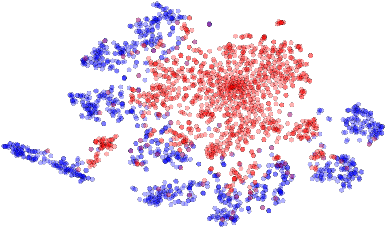
\includegraphics[width=0.45\textwidth]{./figures/adaptation_vis/pool2_mnist2inv_before.pdf}}\hfill%
  \subfigure[Adapted]{%%
    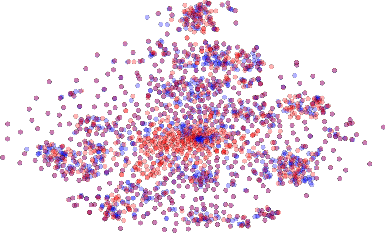
\includegraphics[width=0.45\textwidth]{./figures/adaptation_vis/pool2_mnist2inv_after.pdf}}%%
  \hspace*{\fill}%
  \end{minipage}%
  \begin{minipage}{.5\textwidth}
  \centering
  \small{{\sc Syn Numbers $ \rightarrow $ SVHN}: last hidden layer of the label predictor}
  \setcounter{subfigure}{0}
  \hspace*{\fill}%
  \subfigure[Non-adapted]{%%
    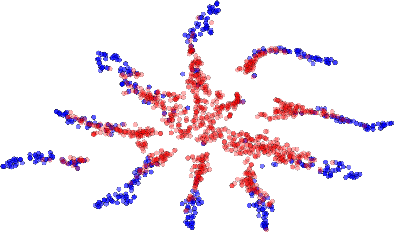
\includegraphics[width=0.45\textwidth]{./figures/adaptation_vis/before.pdf}}\hfill%
  \subfigure[Adapted]{%%
    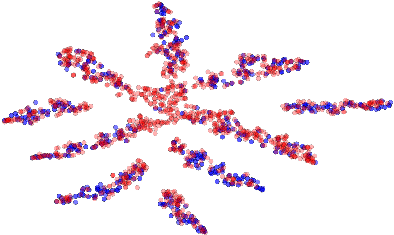
\includegraphics[width=0.45\textwidth]{./figures/adaptation_vis/after.pdf}}%%
  \hspace*{\fill}%
  \end{minipage}
  \caption{The effect of adaptation on the distribution of the extracted features (best viewed in color). The figure shows t-SNE \cite{Maaten13} visualizations of the CNN's activations {\bf (a)} in case when no adaptation was performed and {\bf (b)} in case when our adaptation procedure was incorporated into training. {\it Blue} points correspond to the source domain examples, while {\it red} ones correspond to the target domain. In all cases, the adaptation in our method makes the two distributions of features much closer.}
  \label{fig:exper_adapt_vis}
\end{figure*}

\subsection{Results}
\label{sect:exper_quant}

We now discuss the experimental settings and the results. In each case, we train on the source dataset and test on a different target domain dataset, with considerable shifts between domains (see \fig{exper_domains_examples}). The results are summarized in \tab{results} and \tab{results_office}. 

\vspace{2mm}\noindent {\bf MNIST $ \rightarrow $ MNIST-M.}
Our first experiment deals with the MNIST dataset~\cite{LeCun98} (source). In order to obtain the target domain ({\sc MNIST-M}) we blend digits from the original set over patches randomly extracted from color photos from BSDS500 \cite{Arbelaez11}. This operation is formally defined for two images $ I^{1}, I^{2} $ as $ I_{ijk}^{out} = | I_{ijk}^{1} - I_{ijk}^{2} | $, where $ i, j $ are the coordinates of a pixel and $ k $ is a channel index. In other words, an output sample is produced by taking a patch from a photo and inverting its pixels at positions corresponding to the pixels of a digit. For a human the classification task becomes only slightly harder compared to the original dataset (the digits are still clearly distinguishable) whereas for a CNN trained on MNIST this domain is quite distinct, as the background and the strokes are no longer constant. Consequently, the source-only model performs poorly. Our approach succeeded at aligning feature distributions (\fig{exper_adapt_vis}), which led to successful adaptation results (considering that the adaptation is unsupervised). At the same time, the improvement over source-only model achieved by subspace alignment (SA) \cite{Fernando13} is quite modest, thus highlighting the difficulty of the adaptation task. 

\vspace{2mm}\noindent {\bf Synthetic numbers $ \rightarrow $ SVHN.}
To address a common scenario of training on synthetic data and testing on  real data, we use Street-View House Number dataset {\sc SVHN} \cite{Netzer11} as the target domain and synthetic digits as the source. The latter ({\sc Syn ~Numbers}) consists of ~500,000 images generated by ourselves from Windows fonts by varying the text (that includes different one-, two-, and three-digit numbers), positioning, orientation, background and stroke colors, and the amount of blur. The degrees of variation were chosen manually to simulate SVHN, however the two datasets are still rather distinct, the biggest difference being the structured clutter in the background of SVHN images. 

The proposed backpropagation-based technique works well covering two thirds of the gap between training with source data only and training on target domain data with known target labels. In contrast, SA~\cite{Fernando13} does not result in any significant improvement in the classification accuracy, thus highlighting that the adaptation task is even more challenging than in the case of the MNIST experiment.

\vspace{2mm}\noindent {\bf MNIST $ \leftrightarrow $ SVHN.}
In this experiment, we further increase the gap between distributions, and test on {\sc MNIST} and {\sc SVHN}, which are significantly different in appearance. Training on SVHN even without adaptation is challenging --- classification error stays high during the first 150 epochs. In order to avoid ending up in a poor local minimum we, therefore, do not use learning rate annealing here. Obviously, the two directions ({\sc MNIST} $ \rightarrow $ {\sc SVHN} and {\sc SVHN} $ \rightarrow $ {\sc MNIST}) are not equally difficult. As {\sc SVHN} is more diverse, a model trained on SVHN is expected to be more generic and to perform reasonably on the MNIST dataset. This, indeed, turns out to be the case and is supported by the appearance of the feature distributions. We observe a quite strong separation between the domains when we feed them into the CNN trained solely on { \sc MNIST}, whereas for the {\sc SVHN}-trained network the features are much more intermixed. This difference probably explains why our method succeeded in improving the performance by adaptation in the {\sc SVHN} $ \rightarrow $ {\sc MNIST} scenario (see \tab{results}) but not in the opposite direction (SA is not able to perform adaptation in this case either). Unsupervised adaptation from MNIST to SVHN gives a failure example for our approach (we are unaware of any unsupervised DA methods capable of performing such adaptation).

\vspace{2mm}\noindent {\bf Synthetic Signs $ \rightarrow $ GTSRB.}
Overall, this setting is similar to the {\sc Syn Numbers} $ \rightarrow $ {\sc SVHN} experiment, except the distribution of the features is more complex due to the significantly larger number of classes (43 instead of 10). For the source domain we obtained~100,000 synthetic images (which we call {\sc Syn~Signs}) simulating various photoshooting conditions. Once again, our method achieves a sensible increase in performance once again proving its suitability for the synthetic-to-real data adaptation.

\begin{figure}
  \centering
  \setlength\figureheight{2.7cm}
  \setlength\figurewidth{6.8cm}
  % This file was created by matlab2tikz v0.5.0 running on MATLAB 8.3.
%Copyright (c) 2008--2014, Nico Schlömer <nico.schloemer@gmail.com>
%All rights reserved.
%Minimal pgfplots version: 1.3
%
%The latest updates can be retrieved from
%  http://www.mathworks.com/matlabcentral/fileexchange/22022-matlab2tikz
%where you can also make suggestions and rate matlab2tikz.
%
\begin{tikzpicture}[font=\scriptsize]

\begin{axis}[%
width=0.95092\figurewidth,
height=\figureheight,
at={(0\figurewidth,0\figureheight)},
scale only axis,
xmin=10000,
xmax=50000,
xlabel={Batches seen},
ymin=0,
ymax=1,
ylabel={Validation error},
axis x line*=bottom,
axis y line*=left,
legend style={at={($ (1,1) + (-0.1cm,-0.1cm) $)},anchor=north east,align=left,legend cell align=left,draw=black},
xmajorgrids,
ymajorgrids,
grid style={dashed}
]
\addplot [color=blue,solid,line width=1.0pt]
  table[row sep=crcr]{%
10500	0.199757996632997\\
11000	0.19162984006734\\
11500	0.190788089225589\\
12000	0.192918771043771\\
12500	0.196390993265993\\
13000	0.185527146464646\\
13500	0.190472432659933\\
14000	0.185606060606061\\
14500	0.183422769360269\\
15000	0.189051978114478\\
15500	0.191524621212121\\
16000	0.186079545454545\\
16500	0.179424452861953\\
17000	0.187684132996633\\
17500	0.187868265993266\\
18000	0.180923821548822\\
18500	0.187315867003367\\
19000	0.178661616161616\\
19500	0.18102904040404\\
20000	0.180555555555556\\
20500	0.176662457912458\\
21000	0.183791035353535\\
21500	0.179214015151515\\
22000	0.178898358585859\\
22500	0.178898358585859\\
23000	0.174479166666667\\
23500	0.174742213804714\\
24000	0.171059553872054\\
24500	0.177951388888889\\
25000	0.174794823232323\\
25500	0.174084595959596\\
26000	0.174636994949495\\
26500	0.169034090909091\\
27000	0.171191077441077\\
27500	0.170875420875421\\
28000	0.171506734006734\\
28500	0.170217803030303\\
29000	0.169244528619529\\
29500	0.169875841750842\\
30000	0.168744739057239\\
30500	0.17048085016835\\
31000	0.169454966329966\\
31500	0.167771464646465\\
32000	0.168849957912458\\
32500	0.168323863636364\\
33000	0.168718434343434\\
33500	0.165667087542088\\
34000	0.167376893939394\\
34500	0.169007786195286\\
35000	0.167140151515152\\
35500	0.165667087542088\\
36000	0.167850378787879\\
36500	0.169823232323232\\
37000	0.170691287878788\\
37500	0.16640361952862\\
38000	0.167981902356902\\
38500	0.169875841750842\\
39000	0.166771885521886\\
39500	0.169376052188552\\
40000	0.168087121212121\\
40500	0.165509259259259\\
41000	0.167718855218855\\
41500	0.168060816498317\\
42000	0.166035353535354\\
42500	0.166692971380471\\
43000	0.166429924242424\\
43500	0.167034932659933\\
44000	0.170349326599327\\
44500	0.169744318181818\\
45000	0.168218644781145\\
45500	0.166429924242424\\
46000	0.166324705387205\\
46500	0.168771043771044\\
47000	0.168034511784512\\
47500	0.168718434343434\\
48000	0.171059553872054\\
48500	0.170638678451178\\
49000	0.16819234006734\\
49500	0.168981481481481\\
50000	0.167902988215488\\
};
\addlegendentry{Real data only};

\addplot [color=cyan,solid,line width=1.0pt]
  table[row sep=crcr]{%
10500	0.9625\\
11000	0.79765625\\
11500	0.715625\\
12000	0.6140625\\
12500	0.52109375\\
13000	0.459375\\
13500	0.4484375\\
14000	0.421875\\
14500	0.39453125\\
15000	0.4109375\\
15500	0.34296875\\
16000	0.36875\\
16500	0.3359375\\
17000	0.36171875\\
17500	0.3171875\\
18000	0.3484375\\
18500	0.32421875\\
19000	0.315625\\
19500	0.346875\\
20000	0.31875\\
20500	0.35390625\\
21000	0.3265625\\
21500	0.33359375\\
22000	0.3171875\\
22500	0.28515625\\
23000	0.30546875\\
23500	0.309375\\
24000	0.2796875\\
24500	0.30859375\\
25000	0.30703125\\
25500	0.3078125\\
26000	0.28671875\\
26500	0.2875\\
27000	0.31484375\\
27500	0.2859375\\
28000	0.29375\\
28500	0.31328125\\
29000	0.3078125\\
29500	0.2859375\\
30000	0.2890625\\
30500	0.284375\\
31000	0.2953125\\
31500	0.26953125\\
32000	0.29921875\\
32500	0.30078125\\
33000	0.2640625\\
33500	0.309375\\
34000	0.2734375\\
34500	0.290625\\
35000	0.26796875\\
35500	0.3015625\\
36000	0.26796875\\
36500	0.2921875\\
37000	0.265625\\
37500	0.2765625\\
38000	0.2859375\\
38500	0.32109375\\
39000	0.28046875\\
39500	0.275\\
40000	0.24921875\\
40500	0.29140625\\
41000	0.26640625\\
41500	0.265625\\
42000	0.259375\\
42500	0.2765625\\
43000	0.26796875\\
43500	0.2765625\\
44000	0.27265625\\
44500	0.25546875\\
45000	0.26484375\\
45500	0.271875\\
46000	0.2703125\\
46500	0.26171875\\
47000	0.246875\\
47500	0.25078125\\
48000	0.29609375\\
48500	0.2640625\\
49000	0.26875\\
49500	0.26015625\\
50000	0.2578125\\
};
\addlegendentry{Synthetic data only};

\addplot [color=red,solid,line width=1.0pt]
  table[row sep=crcr]{%
10500	0.943892045454545\\
11000	0.943892045454545\\
11500	0.943892045454545\\
12000	0.943892045454545\\
12500	0.848300715488216\\
13000	0.658722643097643\\
13500	0.590593434343434\\
14000	0.475484006734007\\
14500	0.313946759259259\\
15000	0.235690235690236\\
15500	0.17879313973064\\
16000	0.152383207070707\\
16500	0.12912984006734\\
17000	0.114478114478114\\
17500	0.116214225589226\\
18000	0.1015625\\
18500	0.10066813973064\\
19000	0.101983375420875\\
19500	0.0914351851851852\\
20000	0.0895675505050505\\
20500	0.0894360269360269\\
21000	0.0827283249158249\\
21500	0.0798611111111111\\
22000	0.0859638047138047\\
22500	0.0799137205387205\\
23000	0.0778619528619529\\
23500	0.0737584175084175\\
24000	0.0742582070707071\\
24500	0.0776778198653199\\
25000	0.0771517255892256\\
25500	0.0725747053872054\\
26000	0.0739425505050505\\
26500	0.0734953703703704\\
27000	0.0730744949494949\\
27500	0.0688920454545455\\
28000	0.0702072811447811\\
28500	0.072337962962963\\
29000	0.0670244107744108\\
29500	0.0733638468013468\\
30000	0.0667613636363636\\
30500	0.0692340067340067\\
31000	0.0652093855218855\\
31500	0.0664720117845118\\
32000	0.0655776515151515\\
32500	0.0671296296296296\\
33000	0.0656039562289562\\
33500	0.0646043771043771\\
34000	0.0668665824915825\\
34500	0.0638678451178451\\
35000	0.065077861952862\\
35500	0.0649989478114478\\
36000	0.0672348484848485\\
36500	0.0668665824915825\\
37000	0.0626052188552189\\
37500	0.0652093855218855\\
38000	0.0626315235690236\\
38500	0.0627893518518518\\
39000	0.0613162878787879\\
39500	0.063236531986532\\
40000	0.0629208754208754\\
40500	0.0639467592592593\\
41000	0.0612899831649832\\
41500	0.0653409090909091\\
42000	0.0608691077441077\\
42500	0.0613425925925926\\
43000	0.0630260942760943\\
43500	0.060106271043771\\
44000	0.0638678451178451\\
44500	0.0602377946127946\\
45000	0.0577388468013468\\
45500	0.062684132996633\\
46000	0.0608164983164983\\
46500	0.0603167087542088\\
47000	0.0577651515151515\\
47500	0.0583175505050505\\
48000	0.0591329966329966\\
48500	0.0607112794612795\\
49000	0.0585805976430976\\
49500	0.0583175505050505\\
50000	0.0590540824915825\\
};
\addlegendentry{Both};

\end{axis}
\end{tikzpicture}%
  \caption{Semi-supervised domain adaptation for the traffic signs. As labeled target domain data are shown to the method, it achieves significantly lower error than the model trained on target domain data only or on source domain data only. \vspace{-4mm}}
  \label{fig:exper_semi_test}
\end{figure}

As an additional experiment, we also evaluate the proposed algorithm for semi-supervised domain adaptation, i.e.\ when one is additionally provided with a small amount of labeled target data. For that purpose we split {\sc GTSRB} into the train set (1280 random samples with labels) and the validation set (the rest of the dataset). The validation part is used solely for the evaluation and does not participate in the adaptation. The training procedure changes slightly as the label predictor is now exposed to the target data. \fig{exper_semi_test} shows the change of the validation error throughout the training. While the graph clearly suggests that our method can be used in the semi-supervised setting, thorough verification of semi-supervised setting is left for future work.


\vspace{2mm}\noindent {\bf Office dataset.} 
We finally evaluate our method on {\sc Office} dataset, which is a collection of three distinct domains: {\sc Amazon}, {\sc DSLR}, and {\sc Webcam}. Unlike previously discussed datasets, {\sc Office} is rather small-scale with only 2817 labeled images spread across 31 different categories in the largest domain. The amount of available data is crucial for a successful training of a deep model, hence we opted for the fine-tuning of the CNN pre-trained on the ImageNet \cite{Jia14} as it is done in some recent DA works \cite{Donahue14,Tzeng14,Hoffman14}. We make our approach more comparable with \cite{Tzeng14} by using exactly the same network architecture replacing domain mean-based regularization with the domain classifier.

Following most previous works, we evaluate our method using 5 random splits for each of the 3 transfer tasks commonly used for evaluation. Our training protocol is close to \cite{Tzeng14,Saenko10,Gong12} as we use the same number of labeled source-domain images per category. Unlike those works and similarly to e.g.\ DLID~\cite{Chopra13} we use the whole unlabeled target domain (as the premise of our method is the abundance of unlabeled data in the target domain). Under this transductive setting, our method is able to improve previously-reported state-of-the-art accuracy for unsupervised adaptation very considerably (\tab{results_office}), especially in the most challenging {\sc Amazon} $ \rightarrow $ {\sc Webcam} scenario (the two domains with the largest domain shift).



\section{Discussion}
\label{sec:discussion}
The advantage of the dueling architecture lies partly in its ability to learn the state-value function efficiently.
With every update of the $Q$ values in the dueling architecture,
the value stream ${V}$ is updated -- this contrasts with the updates in a single-stream architecture where only the value for one of the actions is updated, the values for all other actions remain untouched. This more frequent updating of the value stream in our approach allocates more resources to $V$, and thus allows for better approximation of the state values, which in turn need to be accurate for temporal-difference-based methods like Q-learning to work~\cite{SuttonBarto:1998}.
This phenomenon is reflected in the experiments, where the advantage of the dueling architecture over single-stream 	$Q$ networks grows when the number of actions is large.

Furthermore, the differences between $Q$-values for a given state are often very small relative to the magnitude of $Q$.
For example, after training with DDQN on the game of Seaquest, the average action gap (the gap between the $Q$ values of the best and the second best action in a given state) across visited states is roughly $0.04$, whereas the average state value across those states is about $15$.
This difference in scales can lead to small amounts of noise in the updates can lead to reorderings of the actions, and thus make the nearly greedy policy switch abruptly.
The dueling architecture with its separate advantage stream is robust to such effects.


% Max vs. Mean


\section{Conclusions}
\label{sec:conclusion}

We introduced a new neural network architecture that decouples value and advantage in deep $Q$-networks, while sharing a common feature learning module. The new dueling architecture, in combination with some algorithmic improvements, leads to dramatic improvements over existing approaches for deep RL in the challenging Atari domain. The results presented in this paper are the new state-of-the-art in this popular domain. 

% Add after accepted
%\subsubsection*{Acknowledgments}
%We would like to thank Hado van Hasselt, Arthur Guez, Vlad Mnih, Nicolas Hess, Marc Bellemare, Georg Ostrovski, Tom Schaul and all the folks at Google DeepMind for making this possible.


\bibliography{deeprl}
\bibliographystyle{icml2016}

\appendix

\onecolumn
\section{Double DQN Algorithm}
\label{sec:ddqn_alg}
%!TEX root = main.tex
\begin{algorithm2e}[h!]
\small
\SetKwInOut{Input}{input}\SetKwInOut{Output}{output}
\Input{$\mathcal{D}$ -- empty replay buffer; $\theta$ -- initial network parameters, $\theta^-$ -- copy of $\theta$}
\Input{$N_r$ -- replay buffer maximum size; $N_b$ -- training batch size; $N^-$ -- target network replacement freq.}
\For{\mbox{episode} $e \in \{ 1, 2, \ldots, M$ \} } {
  Initialize frame sequence $\mathbf{x} \leftarrow ()$ \;
  \For{$t \in \{ 0, 1, \ldots \} $} {
    Set state $s \leftarrow \mathbf{x}$, sample action $a \sim \pi_\mathcal{B}$ \;
    Sample next frame $x^t$ from environment $\mathcal{E}$ given $(s,a)$ and receive reward $r$, and append $x^t$ to $\mathbf{x}$ \;
    {\bf if} {$|\mathbf{x}| > N_f$} {\bf then} delete oldest frame $x_{t_{min}}$ from $\mathbf{x}$ {\bf end} \;
    Set $s' \leftarrow \mathbf{x}$, and add transition tuple $(s, a, r, s')$ to $\mathcal{D}$,\\~~~~~~~~~replacing the oldest tuple if $|\mathcal{D}| \ge N_r$ \;
    Sample a minibatch of $N_b$ tuples $(s, a, r, s') \sim \mbox{Unif}(\mathcal{D})$\; %uniformly from $\mathcal{D}$ \;
    Construct target values, one for each of the $N_b$ tuples: \;
    Define $a^{\max{}}(s'; \theta) = \argmax_{a'} Q(s', a'; \theta)$\;
    $y_j = \left\{ \begin{array}{ll}
         r & \mbox{if $s'$ is terminal}\\
         r + \gamma Q(s', a^{\max{}}(s'; \theta); \theta^-), & \mbox{otherwise}. \end{array} \right.$ \;
    Do a gradient descent step with loss $\|y_j - Q(s, a ; \theta )\|^2$ \;
    Replace target parameters $\theta^- \leftarrow \theta$ every $N^-$ steps\;
  }
}
\caption{Double DQN Algorithm.}\label{alg:ddqn}
\end{algorithm2e}


%%%%%%%%%%%%%%%%%%%%%%%%%%%%%%%%%%%%%%%%%%%%%%%%%%%%%%%%%%%%%%
%%%%%%%%%%%%%%%%%%%% APPENDIX %%%%%%%%%%%%%%%%%%%%%%%%%%%%%%
%%%%%%%%%%%%%%%%%%%%%%%%%%%%%%%%%%%%%%%%%%%%%%%%%%%%%%%%%%%%%%

\appendix

%\section*{Appendix}

\section{Additional Details on Multi-Scale Processing}
\label{app:detailsMultiscale}

The integration of multi-scale parallel pathways in architectures that use solely unary kernel strides, such as the proposed, was described in Sec.~\ref{subsec:multiscaleCnn}. The required up-sampling of the low-resolution features was performed with simple repetition in our experiments. This was found sufficient, with the following hidden layers learning to combine the multi-scale features. In the case of architectures with strides greater than unary, the last convolutional layers of the two pathways, $L1$ and $L2$, have receptive fields $\boldsymbol{\varphi}_{L1}$ and $\boldsymbol{\varphi}_{L2}$ with strides $\boldsymbol{\tau}_{L1}$ and $\boldsymbol{\tau}_{L2}$ respectively. To preserve spatial correspondence of the multi-scale features and enable the network for dense inference, the dimensions of the input segments should be chosen such that the FMs in $L2$ can be brought to the dimensions of the FMs in $L1$ after sequential resampling by $\uparrow \boldsymbol{\tau}_{L2}$, $\uparrow F_D$, $\downarrow \boldsymbol{\tau}_{L1}$ or equivalent combinations. Here $\uparrow$ and $\downarrow$ represent up- and down-sampling by the given factor. Because they are more reliant on these operations, utilization of more elaborate, learnt upsampling schemes (\cite{Long2014, Ronneberger2015, Noh2015}) should be beneficial in such networks.


\section{Additional Details on Network Configurations}
\label{app:detailsConfig}

\textbf{3D Networks:} The main description of our system is presented in Sec.~\ref{sec:segmentationSystem}. All models discussed in this work outside Sec.~\ref{subsec:val3dContext} are fully 3D CNNs. Their architectures are presented in Table \ref{subtab:netsConfig3d}. They all use the PReLu non-linearity (\cite{he2015delving}). They are trained using the RMSProp optimizer (\cite{rmsProp}) and Nesterov momentum (\cite{sutskever2013importance}) with value $m=0.6$. $L1 = 10^{-6}$ and $L2 = 10^{-4}$ regularisation is applied. We train the networks with dense-training on batches of 10 segments, each of size $25^3$. Exceptions are the experiments in Sec~\ref{subsec:valDenseTraining}, where the batch sizes were adjusted along with the segment sizes, to achieve similar memory footprint and training time per batch. The weights of our shallow, 5-layers networks are initialized by sampling from a normal distribution $\mathcal{N}(0,0.01)$ and their initial learning rate is set to $a=10^{-4}$. Deeper models (and the \quot{Shallow+} model in Sec~\ref{subsec:valDeeper}) use the weight initialisation scheme of \cite{he2015delving}. The scheme increases the signal's variance in our settings, which leads to RMSProm decreasing the effective learning rate. To counter this, we accompany it with an increased initial learning rate $a = 10^{-3}$. Throughout training, the learning rate of all models is halved whenever convergence plateaus. Dropout with 50\% rate is employed on the two last hidden layers of 11-layers deep models.

\textbf{2D Networks:} Table \ref{subtab:netsConfig2d} presents representative examples of 2D configurations that were employed for the experiments discussed in Sec.~\ref{subsec:val3dContext}. Width, depth and batch size were adjusted so that total required memory was similar to the 3D version of DeepMedic. Wider or deeper variants than the ones presented did not show greater performance. A possible reason is that this number of filters is enough for the extraction of the limited 2D information and that the field of view of the deep multi-scale variant is already sufficient for the application. The presented 2D models were regularized with $L1 = 10^{-8}$ and $L2 = 10^{-6}$ since they have less parameters than the 3D variants. All but Dm2dPatch were trained with momentum $m=0.6$ and initial learning rate $a = 10^{-3}$, while the rest with $m=0.9$ and $a = 10^{-2}$ as this setting increased performance. The rest of the hyper parameters are the same as for the 3D DeepMedic.

\setcounter{table}{0}    
\renewcommand\thetable{B.\arabic{table}}

\begin{table}[!h]
\centering
\scriptsize
\caption{Network architectures investigated in Sec.~\ref{sec:vaOfNetArch} and final validation accuracy achieved in the corresponding experiments. (a) 3D and (b) 2D architectures. Columns from left to right: model's name, number of parallel identical pathways and number of feature maps at each of their convolutional layers, number of feature maps at each hidden layer that follows the concatenation of the pathways, dimensions of input segment to the normal and low resolution pathways, batch size and, finally, average DSC achieved on the validation fold. Further configuration details provided in \ref{app:detailsConfig}.}
\label{tab:netsConfig}
\begin{subtable}{1.0\linewidth}
\caption{3D Network Architectures}
\label{subtab:netsConfig3d}
\begin{tabular}{@{}m{1.5cm}m{3.7cm}m{1.2cm}m{1.2cm}m{1.2cm}m{0.8cm}m{1.3cm}}
\toprule	
	               & \#Pathways: FMs/Layer       & FMs/Hidd. & Seg.Norm. & Seg.Low &B.S. & DSC(\%)    \\ \midrule
Shallow(+)         & 1: 30,40,40,50                  & -          & 25x25x25   & -        &10  & 60.2(61.7) \\
Deep(+)            & 1: 30,30,40,40,40,40,50,50      & -          & 25x25x25   & -        &10  & 00.0(64.9)  \\
BigDeep+           & 1: 60,60,80,80,80,80,100,100    & 150,150    & 25x25x25   & -        &10  & 65.2       \\
DeepMedic          & 2: 30,30,40,40,40,40,50,50      & 150,150    & 25x25x25   & 19x19x19 &10  & 66.6       \\ \bottomrule
\end{tabular}
\end{subtable}%
\vspace{10pt}
\begin{subtable}{1.0\linewidth}
\caption{2D Network Architectures}
\label{subtab:netsConfig2d}
\begin{threeparttable}
\begin{tabular}{@{}m{1.5cm}m{3.7cm}m{1.2cm}m{1.2cm}m{1.2cm}m{0.8cm}m{1.3cm}}
\toprule	
	            & \#Pathways: FMs/Layer       & FMs/Hidd. & Seg.Norm. & Seg.Low &B.S. & DSC(\%)    \\ \midrule
%Dm\_3dSeg       & 2: 30,30,40,40,40,40,50,50      & 150,150    & 25x25x17   & 19x19x17   &10 & 62.1       \\
%Dm\_2dPatch 50\% & 2: 30,30,40,40,40,40,50,50      & 150,150    & 17x17x1    & 17x17x1   &540 & 53.7       \\
Dm2dPatch*    	& 2: 30,30,40,40,40,40,50,50      & 150,150    & 17x17x1    & 17x17x1    &540 & 58.8       \\
Dm2dSeg        & 2: 30,30,40,40,40,40,50,50      & 150,150    & 25x25x1    & 19x19x1    &250 & 60.9       \\
Wider2dSeg     & 2: 60,60,80,80,80,80,100,100    & 200,200    & 25x25x1    & 19x19x1    &100 & 61.3       \\
Deeper2dSeg    & 2: 16 layers, linearly 30 to 50 & 150,150    & 41x41x1    & 35x35x1    &100 & 61.5       \\
Large2dSeg  	& 2: 12 layers, linearly 45 to 80 & 200,200    & 33x33x1    & 27x27x1    &100 & 61.3    \\ \bottomrule
\end{tabular}
\begin{tablenotes}
            \item[*] Sampling was manually calibrated to achieve similar class balance as models that are trained on image segments. Model underperformed otherwise.
\end{tablenotes}
\end{threeparttable}
\end{subtable}
\end{table}

\section{Distribution of Tumor Classes Captured in Training}
\label{app:distrTumorClassesTrain}
\setcounter{table}{0}    
\renewcommand\thetable{C.\arabic{table}} 

\hyperref[table:trainingSamplesPercBrats2015Training]{Table C.1}

\begin{table}[!h]
\centering
\scriptsize
\caption{Real distribution of the classes in the training data of BRATS 2015, along with the distribution captured by our proposed training scheme, when segments of size $25^3$ are extracted centred on the tumor and healthy tissue with equal probability. Relative distribution of the foreground classes is closely preserved and the imbalance in comparison to the healthy tissue is automatically alleviated.}
\label{table:trainingSamplesPercBrats2015Training}
\begin{tabular}{@{}lccccc@{}}
\toprule
\multicolumn{1}{c}{} & Healthy		& Necrosis 	& Edema 		& Non-Enh. 	& Enh.Core 	\\ \midrule
Real		 			& 92.42			& 0.43		& 4.87		& 1.02		& 1.27		\\
Captured				& 58.65			& 2.48		& 24.98		& 6.40		& 7.48		\\
\bottomrule
\end{tabular}
\end{table}


% %\newpage
% \section{Score Tables}
% %!TEX root = main.tex
\label{sec:appen}

\begin{table}[h!]
\vspace{-0.25cm}
\caption{Normalized scores, starting with {\bf 30 no-op} actions.}
\footnotesize
\begin{center}
\begin{tabular}{l|rrr}

              Games &      DQN &     DDQN &     Duel \\
              \hline 
               Alien &    20.2\% &    51.0\% &{\bf61.4\%}\\
              Amidar &    56.7\% &   104.3\% &{\bf137.1\%}\\
             Assault &   781.0\% &{\bf995.1\%}&   846.5\% \\
             Asterix &    50.0\% &   206.8\% &{\bf337.4\%}\\
           Asteroids &     1.4\% &     0.0\% &{\bf4.5\%}\\
            Atlantis &  1651.2\% &   576.1\% &{\bf2285.3\%}\\
          Bank Heist &    59.7\% &   137.6\% &{\bf216.2\%}\\
         Battle Zone &    79.1\% &    84.2\% &{\bf99.9\%}\\
          Beam Rider &    49.9\% &{\bf81.0\%}&    71.2\% \\
             Berzerk &    18.4\% &    44.0\% &{\bf53.8\%}\\
             Bowling &    19.8\% &{\bf32.7\%}&    30.8\% \\
              Boxing &   732.5\% &   762.1\% &{\bf827.1\%}\\
            Breakout &  1334.5\% &{\bf1449.2\%}&  1194.5\% \\
           Centipede &    25.9\% &    33.4\% &{\bf55.1\%}\\
     Chopper Command &    80.8\% &    76.0\% &{\bf158.2\%}\\
       Crazy Climber &   399.1\% &   425.2\% &{\bf530.1\%}\\
            Defender &   131.3\% &   205.3\% &{\bf248.8\%}\\
        Demon Attack &   659.6\% &  3182.8\% &{\bf3335.0\%}\\
         Double Dunk &   557.7\% &   607.9\% &{\bf866.5\%}\\
              Enduro &    84.7\% &   140.8\% &{\bf262.4\%}\\
       Fishing Derby &   163.8\% &   202.4\% &{\bf260.7\%}\\
             Freeway &   104.0\% &{\bf112.5\%}&     0.1\% \\
           Frostbite &    17.1\% &    37.9\% &{\bf107.9\%}\\
              Gopher &   395.4\% &   676.7\% &{\bf717.5\%}\\
            Gravitar &     9.4\% &     7.5\% &{\bf13.1\%}\\
            H.E.R.O. &    65.1\% &    64.1\% &{\bf66.4\%}\\
          Ice Hockey &    76.9\% &    70.0\% &{\bf96.4\%}\\
          James Bond &   270.1\% &{\bf485.4\%}&   468.8\% \\
            Kangaroo &   241.6\% &   433.8\% &{\bf496.2\%}\\
               Krull &   639.3\% &   592.3\% &{\bf923.1\%}\\
      Kung-Fu Master &   114.8\% &   131.0\% &{\bf151.4\%}\\
 Montezuma's Revenge &{\bf0.0\%}&     0.0\% &     0.0\% \\
         Ms. Pac-Man &    41.8\% &    36.2\% &{\bf89.9\%}\\
      Name This Game &   102.8\% &   144.6\% &{\bf168.1\%}\\
             Phoenix &   119.2\% &   177.3\% &{\bf344.5\%}\\
            Pitfall! &    -0.8\% &     3.0\% &{\bf3.4\%}\\
                Pong &   114.0\% &   117.8\% &{\bf118.2\%}\\
         Private Eye &{\bf0.2\%}&     0.2\% &     0.1\% \\
              Q*Bert &    97.5\% &   112.3\% &{\bf143.4\%}\\
          River Raid &    38.3\% &    85.8\% &{\bf125.6\%}\\
         Road Runner &   504.7\% &   563.2\% &{\bf887.4\%}\\
            Robotank &   631.5\% &   643.7\% &{\bf645.1\%}\\
            Seaquest &    13.8\% &    39.0\% &{\bf119.5\%}\\
              Skiing &    31.6\% &    63.3\% &{\bf64.6\%}\\
             Solaris &{\bf20.3\%}&    16.5\% &     9.1\% \\
      Space Invaders &   101.6\% &   156.3\% &{\bf412.9\%}\\
         Star Gunner &   559.3\% &   620.5\% &{\bf924.0\%}\\
           Surround  &    26.5\% &    43.2\% &{\bf86.9\%}\\
              Tennis &{\bf231.3\%}&     6.8\% &   186.2\% \\
          Time Pilot &    78.4\% &   287.2\% &{\bf487.5\%}\\
           Tutankham &    36.3\% &{\bf132.5\%}&   128.1\% \\
         Up and Down &    84.7\% &   201.1\% &{\bf397.9\%}\\
             Venture &    13.7\% &     8.3\% &{\bf41.9\%}\\
       Video Pinball &  1113.7\% &{\bf1754.3\%}&   555.9\% \\
       Wizard Of Wor &    51.0\% &   165.2\% &{\bf173.9\%}\\
       Yars' Revenge &    29.1\% &    16.7\% &{\bf90.4\%}\\
              Zaxxon &    58.3\% &   110.8\% &{\bf141.3\%}\\
            \hline
            {\bf Mean}   &    227.9\% & 307.3\% &  {\bf373.1}\% \\
            {\bf Median}   &79.1\% & 117.8\% & {\bf151.4}\% \\
\end{tabular}
\end{center}
\end{table}





\end{document}


% This document was modified from the file originally made available by
% Pat Langley and Andrea Danyluk for ICML-2K. This version was
% created by Lise Getoor and Tobias Scheffer, it was slightly modified
% from the 2010 version by Thorsten Joachims & Johannes Fuernkranz,
% slightly modified from the 2009 version by Kiri Wagstaff and
% Sam Roweis's 2008 version, which is slightly modified from
% Prasad Tadepalli's 2007 version which is a lightly
% changed version of the previous year's version by Andrew Moore,
% which was in turn edited from those of Kristian Kersting and
% Codrina Lauth. Alex Smola contributed to the algorithmic style files.
